\documentclass[12pt]{amsart}
\usepackage{amstext,amsfonts,amssymb,amscd,amsbsy,amsmath,verbatim}
\usepackage[alphabetic,backrefs,lite]{amsrefs} %bibliography
\usepackage{ifthen, fullpage, extarrows}
\usepackage{color,tikz,multirow}
\usepackage{amsthm}
\usepackage{latexsym}
\usepackage[all]{xy}
\usepackage{enumerate}
\usepackage{diagrams}



\newtheorem{lemma}{Lemma}[section]
\newtheorem{theorem}[lemma]{Theorem}
\newtheorem{propo}[lemma]{Proposition}
\newtheorem{prop}[lemma]{Proposition}
\newtheorem{cor}[lemma]{Corollary}
\newtheorem{conj}[lemma]{Conjecture}
\newtheorem{claim}[lemma]{Claim}
\newtheorem{claim*}{Claim}
\newtheorem{thm}[lemma]{Theorem}
\newtheorem{notation}[lemma]{Notation}

\theoremstyle{definition}
\newtheorem{example}[lemma]{Example}
\newtheorem{defn}[lemma]{Definition}

\theoremstyle{remark}
\newtheorem{remark}[lemma]{Remark}
\newtheorem{question}[lemma]{Question}

% Commands

\newcommand{\isom}{\cong}
\newcommand{\m}{\mathfrak m}
\newcommand{\lideal}{\langle}
\newcommand{\rideal}{\rangle}
\newcommand{\initial}{\operatorname{in}}
\newcommand{\Hilb}{\operatorname{Hilb}}
\newcommand{\hilb}{\operatorname{hilb}}
\newcommand{\Spec}{\operatorname{Spec}}
\newcommand{\im}{\operatorname{im}}
\newcommand{\NS}{\operatorname{NS}}
\newcommand{\Frac}{\operatorname{Frac}}
\newcommand{\ch}{\operatorname{char}}
\newcommand{\Proj}{\operatorname{Proj}}
\newcommand{\id}{\operatorname{id}}
\newcommand{\Div}{\operatorname{Div}}
\newcommand{\tr}{\operatorname{tr}}
\newcommand{\Tr}{\operatorname{Tr}}
\newcommand{\supp}{\operatorname{supp}}
\newcommand{\Gal}{\operatorname{Gal}}
\newcommand{\Pic}{\operatorname{Pic}}
\newcommand{\QQbar}{{\overline{\mathbb Q}}}
\newcommand{\Br}{\operatorname{Br}}
\newcommand{\Bl}{\operatorname{Bl}}
\newcommand{\Cox}{\operatorname{Cox}}
\newcommand{\Tor}{\operatorname{Tor}}
\newcommand{\Tot}{\operatorname{Tot}}
\newcommand{\diam}{\operatorname{diam}}
\newcommand{\Hom}{\operatorname{Hom}} %done
\newcommand{\Ext}{\operatorname{Ext}} %done
\newcommand{\sheafHom}{\mathcal{H}om}
\newcommand{\Gr}{\operatorname{Gr}}
\newcommand{\Osh}{{\mathcal O}}
\newcommand{\kk}{\Bbbk}
\newcommand{\coker}{\operatorname{coker}}
\newcommand{\rank}{\operatorname{rank}}
\newcommand{\pt}{\text{pt}}
\newcommand{\codim}{\operatorname{codim}}
\newcommand{\PP}{\mathbb{P}}
\renewcommand{\AA}{\mathbb{A}}
\newcommand{\GG}{\mathbb{G}}
\newcommand{\HH}{\mathrm{H}}
\newcommand{\KK}{\mathrm{K}}
\newcommand{\ZZ}{\mathbb{Z}}
\newcommand{\QQ}{\mathbb{Q}}
\newcommand{\UU}{\mathrm{U}}
\newcommand{\VV}{\mathrm{V}}
\newcommand{\WW}{\mathrm{W}}
\newcommand{\Wvb}{\mathrm{W}_{\text{vb}}}
\newcommand{\NN}{\mathbb{N}}
\newcommand{\CC}{\mathbb{C}}
\newcommand{\RR}{\mathbb{R}}
\newcommand{\bb}{\mathbf{b}}
\newcommand{\bmin}{\mathbf{b}_{\text{min}}}
\newcommand{\bmax}{\mathbf{b}_{\text{max}}}
\newcommand{\uHH}{\underline{\mathsf{H}}}
\newcommand{\cO}{\mathcal{O}}
\newcommand{\cE}{\mathcal{E}}
\newcommand{\cF}{\mathcal{F}}
\newcommand{\cU}{\mathcal{U}}
\newcommand{\EE}{\mathbf{E}}
\newcommand{\bB}{\mathbf{B}}
\newcommand{\bG}{\mathbf{G}}
\newcommand{\bK}{\mathbf{K}}

\newcommand{\FF}{\mathbf{F}}
\newcommand{\Gbull}{\mathbf{G}}
\newcommand{\Kbull}{\mathbf{K}}
\newcommand{\Sym}{\operatorname{Sym}} %done  
\newcommand{\GL}{{GL}}
\newcommand{\Syz}{\operatorname{Syz}}
\newcommand{\pos}{\operatorname{pos}}

\newcommand{\defi}[1]{\textsf{#1}} % for defined terms

\newcommand{\zp}{\circ}
\newcommand{\BQ}{\mathrm{B}}
\newcommand{\DD}{\mathrm{D}}
\newcommand{\w}{\widetilde}
\newcommand{\CQ}{\mathrm{C}}
\newcommand{\CvbQ}{\mathrm{C}_{\text{vb}}}
\newcommand{\BBQ}{\underline{\mathrm{B}}}
\newcommand{\BBirr}{\underline{\mathrm{B}}^{\text{irr}}}
\newcommand{\CCQ}{\underline{\mathrm{C}}}
\newcommand{\Bmod}{\ensuremath{B_\text{mod}}}
\newcommand{\Bint}{\ensuremath{B_\text{int}}}
\newcommand{\Lotimes}{\overset{\mathrm{L}}{\otimes}}
\newcommand{\daniel}[1]{{\color{green} \sf $\clubsuit\clubsuit\clubsuit$ Daniel: [#1]}}
\newcommand{\mauricio}[1]{{\color{blue} \sf $\clubsuit\clubsuit\clubsuit$ Mauricio: [#1]}}
\newcommand{\david}[1]{{\color{red} \sf $\clubsuit\clubsuit\clubsuit$ David: [#1]}}

\renewcommand{\P}{{\mathbb P}}
\def\edim{\operatorname{edim}}
\def\reg{\operatorname{reg}}
\def\pdim{\operatorname{pdim}}
\newcommand{\ve}[1]{\ensuremath{\mathbf{#1}}}
\newcommand{\chr}{\ensuremath{\operatorname{char}}}
\def\brack{[\ , \ ]}
\def\Coh{{\rm Coh}}
\def\gr{{\rm gr}}

\def\ES{Eisenbud-Schreyer}
\def\BS{Boij-S\"oderberg}

\title{Categorified Duality in Boij--S\"oderberg Theory}
\author{David Eisenbud}
\author{Daniel Erman}\thanks{First author supported by an NSF and second author supported by an NSF and by Simons \dots}
\date{\today}
%\address{Department of Mathematics, University of California,
%	Berkeley, CA 94720, USA}
%\email{derman@math.berkeley.edu}
%\urladdr{http://math.berkeley.edu/\~{}derman}



%%%%%%%%%%%%%%%%%%%%%%%%%%%%%%%%%%%%%%%%%%%%%%%%%%%%%%%
%%%%%%%%%%%%%%%%%%%%%%%%%%%%%%%%%%%%%%%%%%%%%%%%%%%%%%%
%%%%%%%%%%%%%%%%%%%%%%%%%%%%%%%%%%%%%%%%%%%%%%%%%%%%%%%
%%%%%%%%%%%%%%%%%%%%%%%%%%%%%%%%%%%%%%%%%%%%%%%%%%%%%%%
\begin{document}
\maketitle



\begin{abstract} Let $\kk$ be a field and let $S = \kk[x_{0}, \dots,x_{n}]$ be the homogeneous coordinate ring of $\PP^{n}_{K}$.
We construct a pairing between derived categories that takes a pair of bounded complexes
finitely generated graded $S$-modules and produces a bounded complex of finitely generated graded modules over a polynomial ring in 1 variable. This pairing simultaneously categorifies all the functionals used by Eisenbud an Schreyer in their proof of the Boij-S\"oderberg conjectures. With this tool we extend the Eisenbud-Schreyer theorem to describe the cone of Betti tables of finite, minimal free complexes of $S$-modules with homology modules of specified dimensions;  and we provide descriptions of cones of Betti tables and cohomology tables in many examples beyond $\PP^n$.
\end{abstract}


%%%%%%%%%%%%%%%%%%%%%%%%%%%%%%%%%%%%%%%%%%%%
%%%%%%%%%%%%%%%%%%%%%%%%%%%%%%%%%%%%%%%%%%%%
\section*{Introduction}
%%%%%%%%%%%%%%%%%%%%%%%%%%%%%%%%%%%%%%%%%%%%
%%%%%%%%%%%%%%%%%%%%%%%%%%%%%%%%%%%%%%%%%%%%
Let $\kk$ be a field, and let $S=\kk[x_0, \dots, x_n]$ be the polynomial ring. Recall that if 
$$
\FF: \cdots \to F_{i}\to \cdots
$$
is a complex of finitely generated graded free $S$-modules, then $\beta_{i,j}\FF$ is by definition the dimension of the degree $j$ component of the graded vector space $H_{i}(F_{i}\otimes_{S}\kk)$. If $\FF$ is bounded, then the \emph{Betti table} of $F$ is the vector with coordinates $\beta_{i,j}\FF$ in the vector space $V = \oplus_{i\in \ZZ} \oplus_{j\in \ZZ}\QQ$. Similarly, the \emph{cohomology table} of a bounded complex of coherent sheaves $\cE$ on $\PP^{n}$ is the vector with coordinates $\gamma_{i,j}\cE := h^{i}\cE(j)$ in the vector space $U = \oplus_{i\in \ZZ}\prod_{j\in \ZZ}\QQ$, where $h^{i}\cE(n)$ denotes the dimension of the $i$-th hypercohomology of the complex $\cE(j) := \cE \otimes \cO_{\PP^{n}}(j)$. Following a common convention we display the Betti table of $\FF$ as a table
of integers where the element of the $i$-th column and $j$-th row is $\beta_{i,i+j}\FF$, and we replace each zeros with $-$. For clarity we often decorate the $(0,0)$ entry
with a superscript $\circ$.
Given a graded module, or a complex of graded modules $M$ over $S$, we write $\widetilde M$ for the corresponding sheaf or complex of sheaves on $\PP^{n}$. 

Eisenbud and Schreyer \cite{eis-schrey1} described an infinite family $\langle -,-\rangle_{\tau,\kappa}$ bilinear functionals that, together, provide a duality between the rational cone generated by the cohomology tables of coherent sheaves on $\PP^n$ on one hand,  and the ratioal cone generated by the Betti tables of minimal free resolutions over the graded polynomial ring $S:=\kk[x_0, \dots, x_n]$ on the other. Using this duality they proved the conjectures of Boij--S\"oderberg \cite{}. The theory has been further extended by ****\david{list some papers}. All these papers use the original functionals $\langle -,-\rangle_{\tau,\kappa}$, but the nature of these functionals has remained mysterious. It has been quite difficult to extend the theory to resolutions over other rings, and only a little progress has been made. \david{papers} Though it seemed natural to try to treat the multi-graded case (Tori varieties!) the goal has been elusive \david{quote Eisenbud-Scheyer...?}

In this paper we interpret all of the functionals $\langle-,-\rangle_{\tau,\kappa}$ in terms of a single a pairing on derived categories. This categorification allows us to extend the theory from free resolutions to the case of finite free complexes with homology. Our theory extends naturally to many other rings, and our pairing admits a simple generalization to the multigraded case.

To be explicit, let $A = \kk[t]$, the polynomial ring in 1 variable and let $D^{b}(\P^{n}), D^{b}(S), D^{b}(A)$ denote the bounded derived categories of the categories of coherent sheaves on $\P^{n}$ and of finitely generated graded modules over $S$ and $A$, respectively.  The central construction of this paper is a functor
$$
D^{b}(S)\times D^{b}(\P^{n})  \rTo^{\Phi} D^{b}(A),
$$
that satisfies the following.
\begin{theorem}\label{thm:Phi}
The functor $\Phi$ has the following  properties:
\begin{enumerate}
	\item\label{thm:Phi:1}  The Betti table of $\Phi(\FF,\cE)$ depends only on the Betti table of $\FF$ and the cohomology table of $\cE$.
	\item\label{thm:Phi:2}  If $\widetilde{\FF}\otimes \cE$ is exact, then $\Phi(\FF,\cE)$ has finite length homology.  This occurs whenever $\FF$ is a complex with finite length homology and $\cE$ is a vector bundle.  More generally, this occurs  whenever  $\FF$ has homology of codimension $\geq \ell$,  $\cE$ has codimension $\geq n+1-\ell$, and $\FF$ and $\cE$ are homologically transverse.
\end{enumerate}
\end{theorem}

The functor $\Phi$ thus yields a bilinear pairing relating Betti tables and cohomology tables.  For instance, one such pairing is given by:
\begin{equation*}%\tag{**}
\label{eqn:**}
%
\left\{\begin{matrix}
%\text{Cone generated by}\\
\text{Betti tables of} \\ \text{free $S$-complexes}\\
\text{ with homology}\\ \text{ of finite length}
\end{matrix}\right\}
%
\times 
%
\left\{\begin{matrix}
%\text{Cone generated by}\\
\text{cohomology }\\
\text{tables of vector}\\
\text{ bundles on } \PP^n
\end{matrix}\right\}
%
\longrightarrow
\left\{\begin{matrix}
%\text{Cone generated by}\\
\text{Betti tables of} \\ \text{free $A$-complexes}\\
\text{ with homology}\\ \text{ of finite length}
\end{matrix}\right\}
\end{equation*}
%(Here we think of a vector bundle
%as a graded module, regarded in turn as a complex of graded modules concentrated in one (arbitrary) homological degree.)
Based on Theorem~\ref{thm:Phi}\eqref{thm:Phi:2}, we also obtain similar pairings where we increase the dimension of the homology of our free $S$-complexes and we correspondingly decrease the dimension of the support of the sheaves on $\mathbb P^n$.  We prove that this pairing gives a  \emph{duality pairing} of cones, as represented in Figure~\ref{fig:bracket},
in the sense that: 
\begin{itemize}
\item It extends to a bilinear pairing $\VV\times \WW\to \UU$.  Further, if we restrict to the convex subcones of $\VV, \WW,$ and $\UU$ generated by the above Betti tables and cohomology tables, then the pairing restricts to a map between these three cones;
\item The only elements of $\VV$ that pair with all elements of the cone in the second factor
 to give elements of the cone in the target are, up to a rational multiple, the Betti tables of  resolutions of finite length modules.  We also obtain a similar statement, where we reverse the roles of 
 the first and second cones.
\end{itemize} 
 We prove similar results for complexes with homology of higher dimension, as well. The case of free resolutions treated in \cite{eis-schrey1} follows immediately by the observation that a  complex of graded free $S$-modules of length $n+1$ with finite length homology has, in fact, homology only at the end, so it is a free resolution (\cite{}).

The target of this duality pairing, the cone of Betti tables on $A$, is easy to describe, and it is easy to write down the positive functionals that define it or the subcone composed of Betti tables of complexes with finite length homology. 
The functor $\Phi$ induces all the pairings defined by Eisenbud and Schreyer: composing $\Phi$ with such functionals we get all the functionals $\langle -,-\rangle_{\tau,\kappa}$ used by Eisenbud and Schreyer.
\begin{figure}
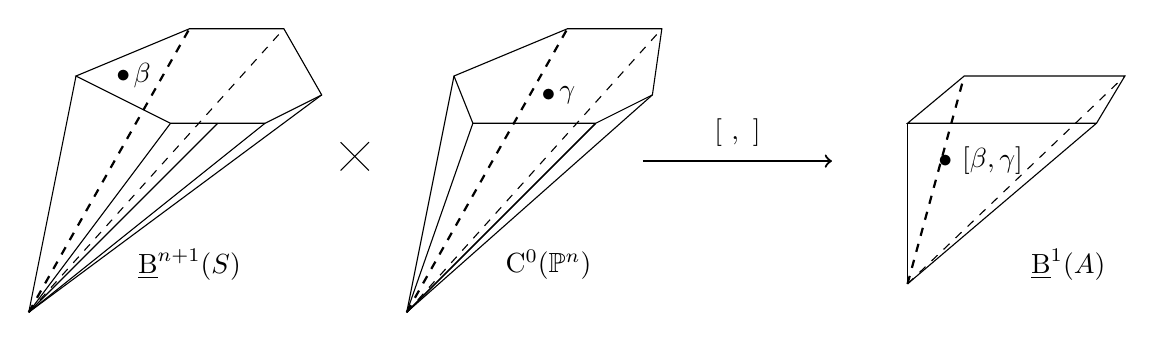
\begin{tikzpicture}[scale=1.2]
%% first cone
\draw[-](.5,.5)--(1,3);
\draw[-](.5,.5)--(2,2.5);
\draw[-](.5,.5)--(3,2.5);
\draw[-](.5,.5)--(3.6,2.8);
\draw[-](.5,.5)--(2.5,2.5);
\draw(1.5,3.0) node {$\bullet$};
\draw(1.7,3.0) node {$\beta$};
\draw(2.2,1.0) node {$\BBQ^{n+1}(S)$};
\draw[dashed,-](.5,.5)--(3.2,3.5);
\draw[dashed,-,thick](.5,.5)--(2.2,3.5);
\draw[-](1,3)--(2,2.5)--(3,2.5)--(3.6,2.8)--(3.2,3.5)--(2.2,3.5)--cycle;
%% the cross
\draw[-] (3.8,2)--(4.1,2.3);
\draw[-] (4.1,2)--(3.8,2.3);
%% second cone
\draw[-](4.5,.5)--(5,3);
\draw[-](4.5,.5)--(5.2,2.5);
\draw(6.0,2.8) node {$\bullet$};
\draw(6.2,2.8) node {$\gamma$};
\draw(6.0,1.0) node {$\CQ^0(\PP^{n})$};
\draw[-](4.5,.5)--(6.5,2.5);
\draw[-](4.5,.5)--(7.1,2.8);
\draw[-](4.5,.5)--(6.5,2.5);
\draw[dashed,-](4.5,.5)--(7.2,3.5);
\draw[dashed,-,thick](4.5,.5)--(6.2,3.5);
\draw[-](5,3)--(5.2,2.5)--(6.5,2.5)--(7.1,2.8)--(7.2,3.5)--(6.2,3.5)--cycle;
%%the arrow
\draw[->,thick](7,2.1)--(9,2.1);
\draw(8,2.4) node {$[\ , \ ]$};
%% third cone
%\draw[-](9.5,.5)--(10,3);
\draw[-](9.8,.8)--(9.8,2.5);
\draw[-](9.8,.8)--(11.8,2.5);
%\draw[-](9.5,.5)--(10.4,2.8);
%\draw[-](9.5,.5)--(11.5,2.5);
\draw[dashed,-](9.8,.8)--(12.1,3.0);
\draw[dashed,-,thick](9.8,.8)--(10.4,3.0);
\draw(10.2,2.1) node {$\bullet$};
\draw(10.7,2.1) node {$[\beta,\gamma]$};
\draw(11.5,1.0) node {$\BBQ^{1}(A)$};
\draw[-](9.8,2.5)--(11.8,2.5)--(12.1,3.0)--(10.4,3.0)--cycle;
\end{tikzpicture}
\caption{Given the Betti table $\beta$ of a complex of free $S$-modules, and the cohomology table $\gamma$ of a coherent sheaf on $\PP^n$, our pairing produces the Betti table $[\beta, \gamma]$ of a complex free $A$-modules.
}
\label{fig:bracket}
\end{figure}

\subsection*{Comparing Complexes and Resolutions} Here is a consequence of the analysis of Betti tables allowed by this categorification: If every bounded complex of free $S$-modules were quasi-isomorphic to its homology---which is not the case except when $n=0$, that is $S$ is the polynomial ring in just 1 variable---then the Betti table of a complex would be the sum of the Betti tables of the resolutions of its homology.  We show that the Betti table is at least a sum of Betti tables of resolutions, but with rational, not integral coefficients, and not necessarily of the original homology modules. Here, for simplicity, are two special cases of this result.
%is the case when the homology has finite length. 

\begin{cor}\label{cor:decompose}
Let $\FF\in \DD^b(S)$.
\begin{enumerate}
	\item  If $\FF$ has finite length homology, then $\beta(\FF)$ may be written as a positive rational combination of Betti tables of shifted free resolutions
	\[\beta(\FF)=\sum_{i=0}^s \beta(M^i)[i]\]
	 where each module $M^i$ has finite length.
	\item  If $\codim H^i\FF\geq i$ then $\beta(\FF)$ may be written as a positive rational combination of Betti tables of shifted free resolutions
\[\beta(\FF)=\sum_{i=0}^s \beta(M^i)[i]\]
where $\codim(M^i)\geq i$ for all $i$.
\end{enumerate}
As in the case of resolutions, the decomposition is algorithmic and, in a certain sense, unique.	
\end{cor}
\begin{cor}\label{cor:decompose}
The Betti table of any bounded graded free complex of $S$-modules, with finite length homology, is a positive rational combination of Betti tables of shifted free resolutions of modules of finite length (as in the case of resolutions, the decomposition is algorithmic and, in a certain sense, unique.)
\end{cor}

The full statement and proof are given in \S\ref{sec:refined}.  \daniel{Need to add some reference to the generalizations.}  The denominators of the coefficients involved in the decomposition may be seen as a measure of the extent to which the complex is not quasi-isomorphic to its homology. 

\begin{example}
Let $S=\kk[x,y]$ and consider the complex:
\[
\FF := \left[S^1\overset{\left(\begin{smallmatrix}x&y\end{smallmatrix}\right)}{\xlongleftarrow{\hspace*{1.1cm}}} S^2(-1)\overset{\left(\begin{smallmatrix}-y^2&xy\\xy&-x^2\end{smallmatrix}\right)}{\xlongleftarrow{\hspace*{1.1cm}}} S^2(-3)\overset{\left(\begin{smallmatrix}y\\x\end{smallmatrix}\right)}{\xlongleftarrow{\hspace*{1.1cm}}} S^1(-4)\right],
\]
which has finite length homology $H_{0}\FF = \kk,\ H_{1}\FF = \kk(-2)$, and the minimal free resolution of $S/(x,y)^{2}$, which 
is
\[
\bG := 
\left[S^1\overset{\left(\begin{smallmatrix}x^{2}&xy&y^{2}\end{smallmatrix}\right)}
{\xlongleftarrow{\hspace*{1.1cm}}} 
S^3(-2)\overset{\left(\begin{smallmatrix}y&0\\-x&y\\0&-x\end{smallmatrix}\right)}{\xlongleftarrow{\hspace*{1.1cm}}} S^2(-3)\right].
\]
The Betti table
$$
\beta(\FF)=\begin{pmatrix} 1^\circ&2&-&-\\-&-&2&1\end{pmatrix}
$$
decomposes as a rational combination of the Betti table of $\bG$ shifted in 
homological degree by 1,
$$
\beta(\bG[1]) =\begin{pmatrix} -^{\circ}&1&-&-\\-&-&3&2\end{pmatrix},
$$
and the Betti table of the dual of $\bG$, 
$$
\beta(\bG^{*}) = \begin{pmatrix} 2^\circ&3&-\\-&-&1\end{pmatrix}.
$$
In fact, as one sees immediately,
\[
\beta(\FF)=
\frac{1}{2}\beta(\bG[1])
+
\frac{1}{2}\beta(\bG^{*}).
\]
By contrast, $\beta(\FF)$ \emph{not} be written as a positive \emph{integral} combination of Betti tables of resolutions of modules of finite length: by Hilbert's Syzygy Theorem the Betti table of $\FF$  is not equal to any Betti table of a resolution, since $\FF$ has length 3; and the sum of the Betti numbers of any resolution of a nonzero module of finite length is at least 4, while the sum of the Betti numbers of $\FF$ is $6<2\cdot 4$.
\end{example}

\begin{example}
Let $S=\kk[x,y,z]$, $I=(x^2,xy,y^2,xz)$, and let $\FF$ be the minimal free resolution of $S/I$.  Since $\FF$ is a resolution, we may apply \cite[Theorem~]{boij-sod2} and decompose
\[
\beta(\FF)=\begin{pmatrix}
1^\zp&-&-&-\\
-&4&4&1
\end{pmatrix}
=
\frac{1}{3}
\begin{pmatrix}
1^\zp&-&-&-\\
-&6&8&3
\end{pmatrix}
+\frac{2}{3}
\begin{pmatrix}
1^\zp&-&-\\
-&3&2
\end{pmatrix}.
\]
On the other hand, we now set $S':=S/(\ell)$, where $\ell$ is a generic linear forms, and we let $\FF'$ be the restriction of $\FF$ to $S'$.  Since $\text{depth}(S/I)=1$, the complex $\FF'$ is not a resolution, but it does have finite length homology.  Hence, applying Corollary~\ref{cor:decompose}, we can decompose $\FF'$ in a different way:
\[
\beta(\FF')=
\begin{pmatrix}
1^\zp&-&-&-\\
-&4&4&1
\end{pmatrix}
=\begin{pmatrix}1^\zp&-&-\\-&3&2\end{pmatrix}
+
3\begin{pmatrix}
-^\zp&-&-&-\\
-&1&2&1
\end{pmatrix}
\] 
\end{example}

%%%%%%%%%%%%%%%%%%%%%%%%%%%%%%
%%%%%%%%%%%%%%%%%%%%%%%%%%%%%%
\subsection*{Beyond Polynomial Rings}
%%%%%%%%%%%%%%%%%%%%%%%%%%%%%%
%%%%%%%%%%%%%%%%%%%%%%%%%%%%%%
It turns out that our description of the cone of Betti tables of bounded complexes
extends to a wide class of rings in the following way. Let $f:X\to \PP^{n}$ be a finite
morphism from a projective variety of dimension $n$, and set $L:=f^*\cO(1)$. 
Write $R=R(X,L)=\oplus_{e\in \mathbb N} H^0(X,L^{\otimes e})$ for the \emph{section ring}
of $L$.

We say that $\cU$ is an \defi{Ulrich sheaf} for $f$ if $f_*(\cU)\cong \cO_{\PP^n}^r$ for some $r>0$.  It was pointed out in \cite[Theorem~5]{eis-schrey-abel} that the existence of an Ulrich sheaf for $f$ implies that  the cone of cohomology tables of vector bundles on $X$ is the same as that on $\PP^{n}$. (The theorem is stated there in the special case when $L$ is very ample, but the proof
carries over to the more general situation.) The situation for Betti tables of resolutions is not at all analogous, but it is analogous for bounded complexes with finite length homology:

%\david{if we compose a finite map with a finte projection we get a finite map with the same $L$
%and the same Ulrich sheaves.
%Couldn't we restrict to this case? Shouldn't we be proving that the cone is the same as
%the cone of complexes with finite homology on $\P^{d}$??}

\begin{cor}\label{cor:isom cones}
If $f:X\to \P^{n}$ is a  finite map from an $n$-dimensional variety and $X$ admits an Ulrich sheaf for $f$, then the cone of Betti tables
of bounded free complexes with finite length homology over  the section ring
of $f^{*}\cO_{\P^{n}}$ is the same
as the cone of complexes with finite length homology  on $S$. 
\end{cor}

 In particular, this Corollary provides the first descriptions of cones of Betti tables over a ring $R$ with a nonstandard grading, as in the following example.

\begin{example}\label{ex:elliptic}
Let $E$ be an elliptic curve and let $L=2P$, where $P$ is any point of $E$.  The map $f$ corresponding to the complete
linear series $|L|$ maps $E$ two-to-one to $\P^{1}$. The ring $R(X,L)$ has the form
$\kk[x_1,x_2,z,w]/(w^{2}-g(x_{1},x_{2})$  where $\deg(x_i)=1, \deg(z)=2$ and $\deg(w)=3$. 
If $p\neq q\in E$ then the sheaf $L(p-q)$ is an Ulrich sheaf for $f$. Thus the cone of
Betti tables of bounded free complexes with finite length homology over $R$ is the same
as the corresponding cone over $\P^{1}$.
\end{example}

Note that, since $f$ is finite, Corollary~\ref{cor:isom cones} implies that $L$ is ample.  However, the theorem is not true for an arbitrary ample divisor.  For instance, let $P$ be a point on an elliptic curve $E$, and let $R=R(E,P)$.  Since $\dim R_1=h^0(E,\cO_E(P))=1$, there cannot exist a pure complex:
\[
0\gets R^1\gets R^2(-1)\gets R(-2)\gets 0
\]
with finite length homology.

For many of the graded rings $R$ covered by Corollary~\ref{cor:isom cones}, there exist finitely generated $R$-modules of infinite projective dimension.  It would  be interesting to consider the cone of Betti tables of unbounded complexes. \david{we could say what we know.}

\subsection*{The Multigraded Case}
The functor $\Phi$ naturally generalizes to the multigraded case, thus providing new possibilities for extending Boij--S\"oderberg theory to toric varieties.  Let $X$ be any projective toric variety with $\rank \Pic(X)=m$.  Let $R$ be the Cox Ring of $X$, presented as an $\mathbb N^m$-graded ring, and let $I$ be the irrelevant ideal of $R$.  We also let $C=\kk[t_1, \dots, t_m]$ by $\mathbb N^m$-graded with irrelevant ideal $(t_1\cdots t_n)$.  We say that a complex $\FF$ has \defi{irrelevant homology} if its homology is supported on the irrelevant ideal.

Use $\DD^b(R)$ and $\DD^b(C)$ to denote the bounded derived categories of finitely generated, multigraded $R$-modules (or $C$-modules).   For $\FF\in \DD^b(R)$ or in $\DD^b(C)$, $i\in \ZZ$, and $\alpha\in \ZZ^m$, we define the multigraded Betti numbers by the formula $\beta_{i,\alpha} \FF:=\dim \Tor_i(\FF,\kk)_{\alpha}$.  Similarly, for $\cE\in \DD^b(X), i\in \ZZ$ and $\alpha\in \ZZ^m$, we define multigraded cohomology numbers by the formula $\gamma_{i,\alpha} \cE:=\dim H^i(X, \cE(\alpha))$.  


For an element $\FF\in \DD^b(R)$ we use $\widetilde{\FF}$ to denote the corresponding complex of coherent sheaves in $\DD^b(X)$.  There exists a functor
\[
\Phi': \DD^b(R)\times \DD^b(X)\to \DD^b(C)
\]
that satisfies the following theorem.
\begin{theorem}\label{thm:Phimulti}
The functor $\Phi'$ has the following  properties:
\begin{enumerate}
	\item\label{thm:Phi':1}  The multigraded Betti table of $\Phi'(\FF,\cE)$ depends only on the multigraded Betti table of $\FF$ and the multigraded cohomology table of $\cE$.
	\item\label{thm:Phi':2}  If $\widetilde{\FF}\otimes \cE$ is exact, then $\Phi(\FF,\cE)$ has irrelevant homology.  This occurs, for instance, whenever $\FF$ is a complex with irrelevant homology and when $\cE$ is a vector bundle.
\end{enumerate}
\end{theorem}



The functor $\Phi'$ thus yields bilinear pairings relating multigraded Betti tables and multigraded cohomology tables, including a pairing of the form:
\begin{equation*}%\tag{**}
\label{eqn:multipairing}
%
\left\{\begin{matrix}
%\text{Cone generated by}\\
\text{Betti tables of} \\ \text{free $R$-complexes with}\\
\text{  irrelevant homology}\end{matrix}\right\}
%
\times 
%
\left\{\begin{matrix}
%\text{Cone generated by}\\
\text{cohomology }\\
\text{tables of vector}\\
\text{ bundles on } X
\end{matrix}\right\}
%
\longrightarrow
\left\{\begin{matrix}
%\text{Cone generated by}\\
\text{Betti tables of} \\ \text{free $C$-complexes with}\\
\text{  irrelevant homology}
\end{matrix}\right\}
\end{equation*}
This opens the door to further toric generalizations of Boij--S\"oderberg theory.  In particular, we remark that the cone of free $C$-complexes with irrelevant homology is far easier to study than the cone of free $C$-complexes with finite length homology.  We expect that the positivity results obtained by applying Theorem~\ref{thm:Phimulti} will play an essential role in toric generalizations of Boij--S\"oderberg theory.



\subsection*{Structure of this paper} The duality pairing is considered in detail in \S\ref{sec:duality pairing}. \david{the rest of this needs to be reconsidered} In \S\ref{sec:PP0} we analyze the cone $\BBQ^1(A)$ in detail, which provides a sort of base case for our positivity and duality statements.  We prove our main results in \S\ref{sec:general case}.  We then briefly discuss applications to the study of free resolutions in \S\ref{sec:refined}.  Finally, in \S\ref{sec:functor}, we extend these results to new polarized varieties and graded rings.

%%%%%%%%%%%%%%%%%%%%%%%%
%%%%%%%%%%%%%%%%%%%%%%%%
\section*{Acknowledgments}
%%%%%%%%%%%%%%%%%%%%%%%%
%%%%%%%%%%%%%%%%%%%%%%%%
We thank Ezra Miller, Christine Berkesch, Ravi Vakil, Rob Lazarsfeld, Bhargav Bhatt,\dots


%%%%%%%%%%%%%%%%%%%%%%%%
%%%%%%%%%%%%%%%%%%%%%%%%
\section{The Pairing $\Phi$}\label{sec:duality pairing}
%%%%%%%%%%%%%%%%%%%%%%%%
%%%%%%%%%%%%%%%%%%%%%%%%

As before, set $A= \kk[t]$. Let 
$\sigma: S\to S\otimes A = S[t]$
be the homomorphism defined by $\sigma(x_{i})=x_{i}t$. 
We write $-\otimes_\sigma S[t]$ to denote tensoring over $S$ with $S[t]$ using the structure
given by $\sigma$. Note that $\sigma$ is not a flat map---it is not even equidimensional.

If $F$ is a graded  $S$-module, then 
$$
F\otimes_{\sigma} S[t]
$$
is a bigraded $S[t]$ module.
Thus we may define a functor $\tau$ on derived
categories that takes a graded complex of free $S$-modules $\FF$ to
$$
\tau(\FF): =\widetilde \FF \otimes_{\sigma}\cO_{\PP^{n}\times \AA^{1}},
$$
a complex of graded sheaves on $\PP^{n}\times \AA^{1}$, with the grading coming from degree in $t$, the coordinate on $\AA^{1}$. For example, if 
$$
\FF: 0\rTo S(-d)\rTo^{f}S\rTo 0
$$
where $f$ is a form of degree $d$, then
$$
\tau(\FF): 0\rTo \cO_{\PP^{n}}(-d)\boxtimes A(-d)\rTo^{t^{d}f}\cO_{\PP^{n}}\boxtimes A \rTo 0
$$
where $P\boxtimes Q$ denotes the tensor product of the pullbacks of $P$ and $Q$ from
$\PP^{n}$ and $\AA^{1}$, respectively. This description of $\tau$ could 
be extended to graded complexes of arbitrary finitely generated graded modules
at the expense of replacing the tensor product with a derived tensor product, but we
will never need this.

%\begin{defn} The functor $\Phi: D^{b}(\P^{n}) \times D^{b}(S) \to D^{b}(A)$ is given by:
%$$
%\Phi(\cE,\FF) = R\pi_{*} \left(\tau_{0}(\cE)\otimes_{\P^{n}\times\AA^{1}} \tau_{1}(\FF)\right)
%$$
%where $\pi: \PP^{n}\times \AA^{1}\to \AA^{1}$ is the projection.
%\end{defn}

\begin{defn} \label{defn:product} The functor $\Phi: \DD^{b}(S)\times \DD^b \to \DD^{b}(A)$ is given by:
$$
\Phi(\FF,\cE) = Rp_{2*} \bigl(\tau(\FF)\otimes_{\P^{n}\times\AA^{1}} (\cE\boxtimes \cO_{\AA^{1}}) \bigr)
$$
where $\FF$ denotes a graded  complex of finitely generated free $S$-modules and
$p_2: \PP^{n}\times \AA^{1}\to \AA^{1}$ is the projection.
\end{defn}


For those comfortable with stacks, Definition~\ref{defn:product}
could be rephrased as follows. Consider the commutative diagram:
\[
\xymatrix{
\PP^n&\PP^{n}\times [\AA^1/\GG_m]\ar[l]_-{\pi_{1}} \ar[r]^-{\Sigma} \ar[d]^{\pi_2}&[\AA^{n+1}/\GG_m]\\
&[\AA^1/\GG_m]&%[\Spec(\kk)/\GG_m]\ar[l]_{o}
}
\]
where $\Sigma$ is the morphism induced by $\sigma$ and the maps $\pi_1$ and $\pi_2$ are the projections.  We could define $\Phi(\FF,\cE)$ to be $R\pi_{2*}\left( \Sigma^*\FF\otimes \pi_{1}^{*}\cE\right)\in \DD^b([\AA^1/\GG_m])$.

To see why this is an equivalent definition, note first  that there is an equivalence of categories (given by pullback/descent) between coherent sheaves on $[\AA^1/\GG_m]$ and graded, finitely generated $A$-modules. Further, since the covering map $\AA^1\to [\AA^1/\GG_m]$ is flat, cohomology commutes with base change (see \cite[0765]{stacks-project}) for the diagram
\[
\xymatrix{
\PP^n\times \AA^1\ar[r]\ar[d]^-{p_2}&\PP^{n}\times [\AA^1/\GG_m]\ar[d]^{\pi_2}\\
\AA^1\ar[r]&[\AA^1/\GG_m].
}
\]
Thus, the pullback of $R\pi_{2*}\left( \Sigma^*\FF\otimes \pi_{1}^{*}\cE\right)$ is quasi-isomorphic 
to $\Phi(\FF,\cE)$ as defined in Definition \ref{defn:product}.

Here is a sample computation of $\Phi$: 

\begin{example} Let 
$$
\bK = \bigl[ S\lTo S^{n+1}(-1) \lTo \wedge^{2}(S^{n+1})(-2) \lTo\cdots\lTo S(-n-1)\bigr]
$$
be the Koszul complex, the minimal free resolution of $\kk$, and take
$\cE = \cO_{\PP^{n}}$, so that 
$$
\bK \cdot \cE = Rp_{2*}\widetilde {\sigma^{*}\bK}.
$$  
There is a spectral sequence converging to $Rp_{2*}(\widetilde {\sigma^{*}\bK})\otimes \cE$
whose $^{2}E$ page has in the $(i,j)$ position the $i$-th homology of the complex
of $j$-th cohomology modules of the terms in $\bK$. But since
$$
\widetilde {\sigma^{*} S(-a)} \cong \cO_{\PP^{n}}(-a)\otimes A(-a),
$$
the terms on this page all vanish except for
$$
H^{0} (\widetilde{\bK_{0}}) = H^{0}(\cO_{\PP^{n}}\boxtimes A) = A,
$$
in cohomological degree 0, and 
$$
H^{n}(\widetilde{\bK_{n+1}}) = H^{n}(\cO_{\PP^{n}}(-n-1)\boxtimes A(-n-1) = A(-n-1)
$$
in cohomological degree $n-(n+1) = -1$.
Thus the complex $\bK \cdot \cE$ has the form
$$
A\lTo^{ut^{n}}A(-n)
$$
for some $u\in \kk$. But the complex $\FF$ has homology of finite length, so the complex $\sigma^{*}\FF \otimes p_{2}^{*}\cE$ has homology annihilated by a power of $t$, and thus $\FF\cdot \cE$ will also have homology annihilated by a power of $t$. It follows that $u\neq 0$, and $\FF\cdot \cO_{\PP^{n}}$ is quasi-isomorphic to the graded $A$-module $A/(t^{n})$, regarded as a complex concentrated in homological degree 0.
\end{example}


%%%%%%%%%%%%%%%%%%%%%%%%
%%%%%%%%%%%%%%%%%%%%%%%%
\section{The Betti table of $\Phi(\FF,\cE)$}\label{sec:duality pairing}
%%%%%%%%%%%%%%%%%%%%%%%%
%%%%%%%%%%%%%%%%%%%%%%%%

\begin{theorem}\label{thm:betti numbers of pairing}
The Betti numbers of $\FF\cdot \cE$ are given by the formula:
\[
\beta_{i,j}(\FF\cdot \cE)=\sum_{p-q=i}  \beta_{p,j}(\FF)\gamma_{q,-j}(\cE).
\]
In particular, the Betti table of $\FF\cdot \cE$ only depends on $\beta(\FF)$ and $\gamma(\cE)$.
\end{theorem}
\begin{proof}
Without loss of generality, we assume that $\FF$ is supported entirely in nonnegative homological degrees, so that $\FF=[\FF_0\gets \dots \gets \FF_p]$.  
We may compute $\FF\cdot \cE$ explicitly in terms of a certain spectral sequence for computing $Rp_{2*}$.  First, we consider the double complex $C_{\bullet, \bullet}$ where $C_{i,\bullet}$ is the Cech resolution of $\widetilde{\FF'}_i\otimes \cE'$ on $\PP^n_A$ with respect to the standard Cech cover of $\mathbb P^n$.  If we represent all of the maps in $C_{\bullet, \bullet}$ with matrices, then all of the vertical maps (which are induced by the Cech resolutions) will involve degree $0$ elements, and all of the horizontal maps (which are induced by the maps in $\rho^*\FF$) will involve bihomogeneous elements that are strictly positive in both bidegrees.

Since $\Tot(C_{\bullet, \bullet})$ is a complex of flat $A$-modules that is quasi-isomorphic to $\FF\cdot \cE$, we can obtain the Betti numbers by computing $\Tor(\Tot(C_{\bullet, \bullet}), A/(t))$.  When we tensor by $A/(t)$, the vertical maps of $C_{\bullet, \bullet}$ are unchanged, but the horizontal maps all go to $0$.  
Hence, one spectral sequence degenerates, so the $i$th homology of $\Tot(C_{\bullet,\bullet})/(t)$ equals the sum 
\[
\HH^i(\Tot(C_{\bullet,\bullet})/(t))\cong \bigoplus_{j} \HH^j_{\text{vert}}(C_{i+j,\bullet})
\]

Now we compute the other spectral sequence.
Recall that $\FF_i=\oplus_{j\in \ZZ} S(-j)^{\beta_{i,j}(\FF)}$.  For brevity, we use $\beta_{i,j}:=\beta_{i,j}(\FF)$, and we may write $\FF_i'\otimes \cE\cong \bigoplus_{j\in \ZZ} \cE(-j)^{\beta_{i,j}}\boxtimes A(-j)^{\beta_{i,j}}$.

After taking the vertical homology of $C_{\bullet, \bullet}$, we obtain:
\[
\xymatrix{
\bigoplus_{j} H^n(\cE(-j)^{\beta_{0,j}})\otimes A(-j)^{\beta_{0,j}}&\bigoplus_{j} H^n(\cE(-j)^{\beta_{1,j}})\otimes A(-j)^{\beta_{1,j}}\ar[l]&\dots\ar[l]\\
\vdots & \vdots&\\
\bigoplus_{j} H^1(\cE(-j)^{\beta_{0,j}})\otimes A(-j)^{\beta_{0,j}}&\bigoplus_{j} H^1(\cE(-j)^{\beta_{1,j}})\otimes A(-j)^{\beta_{1,j}}\ar[l]&\dots\ar[l]\\
\bigoplus_{j} H^0( \cE(-j)^{\beta_{0,j}})\otimes A(-j)^{\beta_{0,j}}&\bigoplus_{j} H^0(\cE(-j)^{\beta_{1,j}})\otimes A(-j)^{\beta_{1,j}}\ar[l]&\dots\ar[l]
}
\]
We conclude that
\[
\Tor^i_A(\FF\cdot \cE, A/(t))\cong \HH^i(\Tot(C_{\bullet,\bullet})/(t))\cong \bigoplus_{p-q=i} \bigoplus_{j} H^q(\cO(-j)^{\beta_{p,j}}\otimes \cE)\otimes A(-j)^{\beta_{p,j}},
\]
which proves the formula.
\end{proof}

There is a simple formula for entries in the Betti table of $\FF\cdot \cE$ in terms of 
the Betti table of $\FF$ and the cohomology table of $\cE$.

We can recover the Betti numbers of a complex $\FF$  or the cohomology
table of a sheaf $\cE$ from the values of the pairing:
\begin{cor} 
\begin{enumerate}
\item 
 $\beta_{i,j}(\FF) = \beta_{i,j}(\Phi(\FF,\cO_{\P^{n}}(j)))$ for all $i$.
\item $h^{i}(\cE(j)) = \beta_{-i,-j}(\Phi(S(j),\cE))$, where $S(j)$ is regarded as a complex concentrated in homological degree 0.
\end{enumerate}\qed
\end{cor}


We will focus in this paper on free complexes, and we will need to use the definition of $\Phi$
only in the special case where $\cE$ is a vector bundle, or more generally a sheaf that is \emph{homologically transverse} to $\FF$, in the sense
that $\widetilde \FF\otimes \cE $ is exact, and we will often apply the following easy result:

\begin{prop}
If $\FF$ is a bounded graded free complex, and $\cE$ is a sheaf such that $\widetilde \FF\otimes \cE$ is exact, then the homology of the complex $\Phi(\FF,\cE)$ has finite length.
\end{prop}

\begin{proof} It suffices to show that the homology of $\Phi(\FF,\cE)$ is annihilated by
a power of $t$. After inverting $t$ the map $\sigma$ becomes the usual inclusion $S\subset S[t,t^{-1}]$
composed with the invertible change of variables $x_{i}\mapsto x_{i}t$. Thus the complex 
$$
\Gbull:=\bigl(\widetilde\FF\otimes_{\sigma}\cO_{\PP^{n}\times \Spec A[t,t^{-1}]}\bigr)
\otimes_{\PP^{n}\times \Spec A[t,t^{-1}]}
\cE \cong \widetilde \FF \otimes \cE \otimes \cO_{\Spec A[t,t^{-1}]}
$$
has no homology. It follows by a spectral sequence computation that 
the complex $R\pi_{2*}\GG$ on $\Spec A[t,t^{-1}]$ has no homology. By flat base change,
this is equal to the restriction of $\Phi(\FF,\cE)$ on the open set $t^{-1}$, and we see that the homology
of $\Phi(\FF,\cE)$ is annihilated by a power of $t$, as required.
\end{proof}


\david{untouched after here on March 1}
We use the notation $[\FF,\cF]$ to denote the Betti table of the complex $\FF\cdot \cF$, i.e.:
\[
[\FF,\cF]:=\beta( \FF\cdot \cF).
\]
Let $\eta: \Spec(\kk)\to [\AA^1/\GG_m]$ be the generic point.  Then $\eta^*(\FF\cdot \cF)$ is simply isomorphic to $Rp_{2*}(\FF\otimes \cF)$ (by flat base change and the fact that $\eta$ is a section of the structure map $[\AA^1/\GG_m]\to \Spec(\kk)$).  Thus, if $\FF\otimes \cF$ is exact on $\PP^n$, then $\FF\cdot \cF$ has finite length homology on $\Spec(A)$.

It follows that the map in \eqref{eqn:pairing} is well-defined.  Namely, if $\FF\in \BBQ^k(\PP^n)$ and $\cF\in \CQ^{n+1-k}(\PP^n)$, then (after possibly acting on $\FF$ or $\cF$ by an automorphism of $\PP^n$) we can assume that $\FF$ and $\cF$ are homologically transverse, and thus that $\FF\otimes \cF$ is an exact complex.  It then follows that $\FF\cdot \cF$ is a complex with finite length homology, and thus that $[\FF, \cF]\in \BBQ^1(A)$.  The fact that $[\FF,\cF]$ only depends on $\beta(\FF)$ and $\gamma(\cF)$ follows from Lemma~\ref{lem:product is a complex}.


\begin{example}
Let $S=\kk[x_1,x_2, x_3]$ and let $\FF$ be a positive, free complex with
\[
\beta(\FF)=\begin{pmatrix} 4&8&6&-\\-&6&8&4\end{pmatrix}
\]
%of the form:
%\[
%\FF=\left[\underline{{S}}^4 \gets \begin{matrix} S^8(-1)\\ \oplus \\ S^6(-2)\end{matrix}\gets  \begin{matrix} S^6(-2)\\ \oplus \\ S^8(-3)\end{matrix}
%\gets S^4(-4)\gets 0.\right]
%\]
%Then $\FF\cdot \cO_{\PP^2}$ is a complex of the form:
%\[
%\FF\cdot \cF
%%=\left[\begin{matrix} \underline{A}\otimes_{\kk} H^0(\cO^4)\\ \oplus \\ A(-3)\otimes_{\kk} H^2(\cO(-3)^8) \end{matrix}\gets A(-4)\otimes_{\kk} H^2(\cO(-4)^4)\gets 0\right
%=\left[ \begin{matrix} A^4\\ \oplus \\ A^8(-3) \end{matrix} \gets A^{12}(-4)\right].
%\]
Let $\cE$ be a rank $2$ supernatural bundle of type $(0,-4)$, so that
\[
\gamma(\cE)=
\begin{vmatrix}
\dots&21&12&5&-&-&-&-&-&\dots\\
\dots&-&-&-&3&4&3&-&-&\dots\\
\dots&-&-&-&-&-&-^\circ&5&12&\dots
\end{vmatrix}
\]
We then have
\[
[\FF, \cE]=
\begin{pmatrix}
-&-^\circ\\
24&24\\
24&24
\end{pmatrix}.
\]
\end{example}

%%%%%%%%%%%%%%%%%%%%%%%%
%%%%%%%%%%%%%%%%%%%%%%%%
\section{The structure of $\DD^b(A)$}\label{sec:DbA}
%%%%%%%%%%%%%%%%%%%%%%%%
%%%%%%%%%%%%%%%%%%%%%%%%
We now turn to the target of $\Phi$, the bounded derived category $\DD^b(A)$ of the category of 
complexes of finitely generated $A = \kk[t]$-modules, and the cone of Betti tables of complexes
with finite length homology inside it.

Because the global dimension of $A$ is 1, the structure of $\DD^b(A)$ is simple: any element $\Gbull\in \DD^b(A)$ is quasi-isomorphic to its homology, and the homology $\HH(\Gbull)$ decomposes as
\[
\HH(\Gbull)=\left( \bigoplus_{i,j\in \ZZ} A(-j)[i]^{\lambda_{i,j}(\Gbull)}\right) \bigoplus \left( \bigoplus_{\substack{i,j\in \ZZ\\ k\in \ZZ_{>0}}} (A(-j)[i]/t^k)^{\nu_{i,j,k}(\Gbull)}\right),
\]
for uniquely defined nonnegative integers $\lambda_{i,j}(\Gbull), \nu_{i,j,k}(\Gbull)$.  Hence, as a monoid with respect to direct sum, $\DD^b(A)$ is isomorphic to a free abelian monoid on the countable set of generators $\{\lambda_{i,j} | i,j\in \ZZ\} \cup \{ \nu_{i,j,k}  | i,j\in \ZZ, k\in \ZZ_{>0}\}$. 

Note that a complex $\Gbull$ has finite length homology if and only if $\lambda_{i,j}(\Gbull)=0$ for all $i,j$.  We  define $\DD^b(A)_{\text{tor}}$ as the subcategory of complexes $\Gbull$ where $\lambda_{i,j}(\Gbull)=0$.  We use $\DD^b(A)\otimes_{\ZZ} \QQ$ and $\DD^b(A)_{\text{tor}}\otimes_{\ZZ} \QQ$ for the associated vector spaces.


%%%%%%%%%%%%%%%%%%%%%%%%
%%%%%%%%%%%%%%%%%%%%%%%%
\subsection{Complexes on $A$ with finite length homology}\label{sec:PP0}
%%%%%%%%%%%%%%%%%%%%%%%%
%%%%%%%%%%%%%%%%%%%%%%%%
Let $B^{1}(A)$ be the cone of Betti tables of bounded free complexes over $A$ with 
homology of codimension 1---that is to say, with finite length homology. \david{this notation has
not been introduced in general yet---do it again when we come to $B^{c}(S)$.}

\begin{prop}\label{prop:conePP0}
There is a natural bijection
\[
\left\{
\begin{matrix}
\text{Extremal rays of }\\
\text{the cone } \BBQ^{1}(A)
\end{matrix}
\right\}
\longleftrightarrow
\left\{
\begin{matrix}
\text{Shifted degree sequences }\\
\text{ of codimension $1$}
\end{matrix}
\right\}.
\]
Further, $\BBQ^1(A)$ has the structure of a simplicial fan, where simplices correspond to chain of shifted degree sequences.  
\end{prop}
This proposition also leads to a description of the nonnegative linear functionals on $\BBQ^1(A)$.  To give this halfspace description, we now introduce a graded variant of a partial Euler characteristic.  Given a Betti table in $\UU$, we define $\chi_{\tau,\kappa}$ as the dot product of that Betti table with:
\[
\chi_{\tau,\kappa}:=
\left(
\begin{array}{cccccccc}
 & \vdots& &\multicolumn{1}{|c}{\vdots}&& \vdots&&\\
\dots&0&0&\multicolumn{1}{|c}{1}&-1&1&-1&\dots\\
\dots&0&0&\multicolumn{1}{|c}{1}&-1&1&-1&\dots\\
\dots&0&0&\multicolumn{1}{|c}{\mathbf{1}}&-1&1&-1&\dots\\ \cline{4-5}
\dots&0&0&0&0&\multicolumn{1}{|c}{1}&-1&\dots\\
\dots&0&0&0&0&\multicolumn{1}{|c}{1}&-1&\dots\\
& \vdots&&\vdots&& \multicolumn{1}{|c}{\vdots}&&\\
\end{array}
\right)
\]
where the boldface $1$ corresponds $\beta_{\tau,\kappa}$, i.e. the boldface $1$ is in column $\tau$ and row $\tau-\kappa$. The line the snakes through
the table indicates how $\chi_{\tau,\kappa}$ separates a Betti into two regions.  In the upper region, this is simply computing an Euler characteristic, and in the lower region, it is dot product with the zero matrix.
%We use the notation $\chi_{\tau,\kappa}$ to suggest that these functionals are  graded variants of the partial Euler characteristic functionals.  
The functional $\chi_{\tau,\kappa}$ is nonnegative for any complex $\Gbull$ with finite length homology.  
\begin{lemma}\label{lem:chi nonneg}
Let $\Gbull\in \DD^b(A)$.  If $\Gbull$ has finite length homology, then:
\[
\chi_{\tau,\kappa}(\Gbull)=\sum_{\substack{j,k \\ j< \kappa+1<j+k}} \nu_{\tau,j,k}(\Gbull) + \sum_{\substack{j,k \\ j> \kappa+1}} \nu_{\tau+1,j,k}(\Gbull).
\]
In particular, $\chi_{\tau,\kappa}(\Gbull)\geq 0$.
\end{lemma}
\begin{proof}
It suffices to evaluate both sides of the equation on $1$-term complexes $A(i)[j]/t^k$, for all $i,j\in \ZZ$ and $k\in \ZZ_{>0}$, and the statement then follows.
\end{proof}

A halfspace description of $\BBQ^1(A)$ only involves individual Betti numbers and these graded partial Euler characteristics.

\begin{cor}\label{cor:dualconeA}
A point $u\in \UU$ lies in $\BBQ^1(A)$ if and only if $u$ satisfies:
	\begin{enumerate}
		\item $\chi(u)= 0$.
		\item $\beta_{i,j}(u)\geq 0$ for all $i,j\in \ZZ$.
		\item  $\chi_{i,j}(u)\geq 0$ for all $i\in \ZZ$ and $j\in \ZZ$.
	\end{enumerate}
\end{cor}

\begin{proof}[Proof of Proposition~\ref{prop:conePP0} and Corollary~\ref{cor:dualconeA}]
The extremal ray description of $\BBQ^1(A)$ is straightforward.  Namely, the cone $\BBQ^1(A)$ is, by definition, the image of the first orthant of $\DD^b(A)_{\text{tor}}\otimes_{\ZZ} \QQ$ under the map of vector space
\[
\DD^b(A)_{\text{tor}}\otimes_{\ZZ} \QQ\to U
\]
that sends a complex $\Gbull$ to its Betti table.  Since each generator of $\DD^b(A)_{\text{tor}}$ maps to a distinct extremal ray of $\BBQ^1(A)$, and since there is a natural bijection between the generators of  $\DD^b(A)_{\text{tor}}$ and the shifted degree sequence $d$ of codimension $1$, this immediately proves the bijection stated in Proposition~\ref{prop:conePP0}.
In addition, Lemma~\ref{lem:chi nonneg} implies that each functional in Corollary~\ref{cor:dualconeA} is nonnegative on $\BBQ^1(A)$.  

To obtain the remaining results, it suffices to show that, if a point $u\in \UU$ satisfies the inequalities in Corollary~\ref{cor:dualconeA}, then we may write $u$ uniquely as a sum of pure tables whose degree sequences form a chain.  It suffices to consider points $u\in \UU$ whose entries are all integral and which have no common factor.  Since all entries of $u$ must be nonnegative, we will then induct on the sum of all of the entries of $u$.  When all entries of $u$ are zero, then $u$ is the empty sum of pure diagrams, and this provides our base case.

Otherwise, $u$ has some nonzero entry.  We fix $(a,b)$ so that $u_{a,b}$ is the top nonzero entry in the rightmost nonzero column of $u$.  We then set $c$ so that $u_{a-1,c}$ is the top nonzero entry in column $a-1$.  We claim that, $c<b$, i.e. that $u$ has the form:
\[
u=
\left(
\begin{array}{ccccccc}
 & \vdots& \multicolumn{1}{|c}{\vdots}&\vdots& \vdots&&\\
\dots&u_{a-2,c-2}&\multicolumn{1}{|c}{0}&0&0&\dots\\
\dots&u_{a-2,c-1}&\multicolumn{1}{|c}{u_{a-1,c}}&0&0&\dots\\
 & \vdots& \multicolumn{1}{|c}{\vdots}&\vdots& \vdots&&\\
%\dots&u_{a-2,b-4}&u_{a-1,b-3}&0&0&\dots\\
\dots&u_{a-2,b-3}&\multicolumn{1}{|c}{u_{a-1,b-2}}&0&0&\dots\\
\dots&u_{a-2,b-2}&\multicolumn{1}{|c}{u_{a-1,b-1}}&u_{a,b}&0&\dots\\ \cline{3-4}
\dots&u_{a-2,b-1}&u_{a-1,b}&u_{a,b+1}&\multicolumn{1}{|c}{0}&\dots\\
%\dots&u_{a-2,b}&u_{a-1,b+1}&u_{a,b+2}&0&\dots\\
& \vdots&\vdots&\vdots& \multicolumn{1}{|c}{\vdots}&&\\
\end{array}\right).
\]
The claim follows from the fact that $\chi_{a-1,b-1}(u)\geq 0$.  Namely, computing $\chi_{a-1,b-1}(u)$
is the same as computing the Euler characteristic of the region that lies above the line.  Since this must be nonnegative,
it follows that $c<b$.

We now set
\[
u':=u-\beta(A(-c)[-a+1]/t^{b-c}).
\]
Since $u$ satisfies the inequalities in Corollary~\ref{cor:dualconeA}, one may verify directly that so does $u'$.  Hence, the induction hypothesis guarantees that we can write $u'$ uniquely as a sum of pure tables whose degree sequences form a chain.  Further, the degree sequence corresponding to $\beta(A(-c)[-a+1]/t^{b-c})$ is less than or equal to any degree sequence that could possibly arise in the decomposition of $u'$, and hence we can use the decomposition of $u'$ to conclude that $u$ decomposes uniquely as a sum of pure tables whose degree sequences form a chain.
\end{proof}

%%%%%%%%%%%%%%%%%%%%%%%%%%%%%%%%%%%%%%%%%
%%%%%%%%%%%%%%%%%%%%%%%%%%%%%%%%%%%%%%%%%
\section{Cones}
%%%%%%%%%%%%%%%%%%%%%%%%%%%%%%%%%%%%%%%%%
%%%%%%%%%%%%%%%%%%%%%%%%%%%%%%%%%%%%%%%%%
\david{This is material from the former intro. I'm not sure we need much of it, since it
is nearly a repeat of what's in the intro now plus what's in \cite{eis-schrey1}. But I haven't
tried to cut it yet.}

\subsection{Duality of Cones of Betti tables and Cohomology Tables}
The notions of Betti tables and cohomology tables extend to the appropriate derived categories.  For any $\FF\in \DD^b(S)$, we define the graded Betti numbers $\beta_{i,j}(\FF):= \dim_\kk \Tor^S_i(\FF,\kk)_j$.  Similarly, we define  $\gamma_{i,j}\cE$, for any bounded complex of coherent sheaves $\cE$, to be the dimension of the $i$-hypercohomology  of $\cE(j)$.

\david{Do we really need the underlines in these definitions?? Is plain $B$ something else?}
\begin{defn}  We define the following cones:
\begin{enumerate}
	\item $\BBQ^{k}(S)\subseteq \VV$ is the convex cone spanned by Betti tables $\beta(\FF)$ as $\FF$ varies over all complexes whose homology modules have codimension at least $k$, for $k=0, \dots, n+1$.
	\item $\CQ^{k}(\PP^n)\subseteq \WW$ is the closure of the convex cone spanned by $\gamma(\cE)$ as $\cE$ varies over all coherent sheaves whose support has codimension at least $k$, for $k=0, \dots, n$.
	\item  $\BBQ^{k}(A)\subseteq \UU$ is the convex cone spanned by $\beta(\Gbull)$ as $\Gbull$ varies over all complexes of $A$-modules whose homology modules have codimension at least $k$, for $k=0,1$. 
\end{enumerate}
\end{defn}

In Theorem~\ref{thm:betti numbers of pairing}, we show that the pairing \eqref{eqn:duality pairing} provides the bilinear map of vector spaces alluded to in \eqref{eqn:**}:
\begin{align*}
\VV\times \WW & \to \UU\\
(\beta(\FF),\gamma(\cE))&\mapsto \beta(\FF\cdot \cE).
\end{align*}
%induces the pairing \eqref{eqn:**} by the formula:
%\[
%(\beta(\FF),\gamma(\cE))\mapsto \beta(\FF\cdot \cE).
%\]
This yields a map between three cones of interest, as illustrated in Figure~\ref{fig:bracket}.
\begin{thm}[Positivity]\label{thm:pos}
If $\widetilde{\FF} \otimes \cE$ is exact on $\PP^n$, then $\FF\cdot \cE$ has finite length homology.  In particular,
for any $\ell=1, \dots, n+1$, the pairing from \eqref{eqn:**} yields a map of cones
\[
\BBQ^{\ell}(S)\times \CQ^{n+1-\ell}(\PP^n)\to \BBQ^1(A).
\]
\end{thm}

This explains some of the mysteries raised by~\cite{eis-schrey1}.  Most notably, each nonnegative functional on Betti tables from \cite[\S4]{eis-schrey1} may be realized via the map:
\[
\beta(\FF)\mapsto \chi_{\tau,\kappa}(\FF\cdot \cE),
\]
where $\cE$ is some vector bundle and where $\chi_{\tau,\kappa}$ is a graded partial Euler characteristic (see \S\ref{sec:PP0}).
A similar statement holds for each nonnegative functional on cohomology tables.  Thus, our duality pairing provides a unifying view on all of the Eisenbud--Schreyer functionals and on the corresponding positivity results, including~\cite[Positivity 1]{eis-schrey-icm} and~ \cite[Positivity 2]{eis-schrey-icm}.  See Lemma~\ref{lem:tau kappa} for a detailed comparison.

Further, this clarifies the duality properties of our cones, although the fact that $\WW$ is an infinite direct product complicates the picture a bit.  See Remark~\ref{rmk:issues} for some discussion of these subtleties.  Fortunately, as shown in \cite{eis-schrey1}, it turns out that the study of $\BBQ^{n+1}(S)$ only requires functionals coming from the cohomology tables of vector bundles.  We thus define $\CvbQ(\PP^n)$ as the subcone of $\WW$ generated by cohomology tables of vector bundles, and we define $\Wvb\subseteq \WW$ as the subspace spanned by the points of $\Wvb$.
For the more general case of $\BBQ^{\ell}(S)$, we fix a linear subspace $\PP^{\ell-1}\subseteq \PP^n$, and we define $\Wvb^{\ell-1}\subseteq \WW$ as the subspace spanned by $\CvbQ(\PP^{\ell-1})$ inside of $\WW$.

With notation as above, let $\mathfrak m:=(x_0, \dots, x_n)$ be the homogeneous maximal ideal of $S$.  To simplify the language of this paper we say that
a free complex $\FF$ over $S$ is \emph{positive} if it is a graded, bounded,
and \emph{minimal} in the sense that $\im \phi_{i}\subseteq \mathfrak m \FF_{i-1}$ for each $i$. 


\begin{thm}[Duality]\label{thm:dual}
We have the following equivalences:
\begin{enumerate}
	\item  A point $v\in \VV$ lies in $\BBQ^{\ell}(S)$ if and only if $[v,\gamma(\cE)]\in \BBQ^1(A)$ for all vector bundles $\cE$ on the linear subspace $\PP^{\ell-1}\subseteq \PP^n$.
	\item  A point $w\in \Wvb^{\ell-1}$ lies in $\CvbQ(\PP^{\ell-1})$ if and only if $[\beta(\FF),w]\in \BBQ^1(A)$ for all positive, free complexes $\FF$ whose homology modules have codimension at least $\ell$.
\end{enumerate}
\[
\BBQ^{\ell}(S)
%=\left\{ \begin{matrix} v\in \VV  \text{ such that }  \\ [v,w] \text{ lies in } \BBQ^1(A) \\ \text{ for all } w\in \CvbQ(\PP^{\ell-1})\end{matrix} \right\}
=\left\{ \begin{matrix} v\in \VV  \text{ such that } [v,\gamma(\cE)]\in \BBQ^1(A) \\ \text{ for all } \gamma(\cE)\in \CvbQ(\PP^{\ell-1})\end{matrix} \right\}
\quad
\text{ and }
\quad
\CvbQ(\PP^{\ell-1})=\left\{ \begin{matrix} w\in \Wvb ^{\ell-1} \text{ such that }  \\ [v,w] \text{ lies in } \BBQ^1(A) \\  \text{ for all } w\in \BBQ^{n+1}(S)\end{matrix} \right\}.
\]
\end{thm}

Theorems~\ref{thm:pos} and \ref{thm:dual} also represent a shift in perspective for Boij--S\"oderberg theory.  Previous work on Boij-S\"oderberg theory focused on resolutions, but we consider more general complexes.  This shift is essential, as the duality pairing does not respect the property of being a resolution: if $\FF$ is a resolution of a finite length module, then $\FF\cdot \cE$ will be a complex of $A$-modules with finite length homology, but it will generally fail to be a resolution.  

Nevertheless, when restricted to resolutions this pairing still yields important information.  As already noted, Theorem~\ref{thm:pos} is sufficiently strong to recover all of the positivity results from \cite{eis-schrey1}.  A minor variant of Theorem~\ref{thm:pos}, which will appear in \cite{eis-erm-refined}, is sufficiently strong to recover the key positivity results from \cite{boij-sod2} and \cite{eis-schrey2}.

%
%%%%%%%%%%%%%%%%%%%%%%%%%
%%%%%%%%%%%%%%%%%%%%%%%%
\subsection{Decomposing the Betti table of a free complex}
%%%%%%%%%%%%%%%%%%%%%%%%
%%%%%%%%%%%%%%%%%%%%%%%%
Our positivity results also lead to an extremal ray description of $\BBQ^{\ell}(S)$ that extends~\cite[Theorem~0.2]{eis-schrey1}.  Since we have expanded our domain from minimal free resolutions to more general complexes, we must allow new extremal rays.  This motivates the following redefinition of the notion of a degree sequence.

\begin{defn}
A \defi{degree sequence of codimension $\ell$} is a sequence
\[d=(\dots, d_i, d_{i+1}, \dots)\in \bigoplus_{\ZZ} \left(\ZZ\cup \{ \pm \infty\}\right) \quad \text{  with } d_i+1\leq d_{i+1},
\]
where there are precisely $\ell+1$ entries of $d$ lying in $\ZZ$.   
%When relevant, we mark the $d_0$ entry by an asterisk.  For example
%\[
%(\dots, 0,3^*,7,\dots),
%\]
%be a degree sequence with $d_0=3$.
\end{defn}
We define a partial order on shifted degree sequences by the termwise partial order, so $d\leq d'$ if $d_i\leq d_i'$ for all $i$.


\begin{notation}
Throughout, we use an asterisk to indicate homological position zero when writing a degree sequence and to indicate position $(0,0)$ when writing a Betti table or a cohomology table.  For example, we write $d=(\dots, -\infty, 0^*,1,2,\infty, \dots)$ for the degree sequence $d_{-1}=-\infty, d_0=0,$ and so on.
\end{notation}


Given any degree sequence $d$, we say that a complex $\FF$ is \defi{pure of type $d$} if, for all $i$ such that $d_i\in \ZZ$, the free module $\FF_i$ is generated entirely in degree $d_i$.  We say that a complex $\FF$ is \defi{Cohen-Macaulay of codimension $\ell$} if each of its nonzero homology modules is Cohen-Macaulay of codimension $\ell$. The existence of pure resolutions (see~\cite{efw} or \cite[\S5]{eis-schrey1}) shows that, for any shifted degree sequence $d$ of codimension $\ell$, there exists a pure, Cohen-Macaulay complex $\FF$ of type $d$ and codimension $\ell$ (which is automatically a resolution).

\begin{thm}[Extremal Rays]\label{thm:extremal rays}
There is a natural bijection:
\[
\left\{
\begin{matrix}
\text{Extremal rays of }\\
\text{the cone } \BBQ^{\ell}(S)
\end{matrix}
\right\}
\longleftrightarrow
\left\{
\begin{matrix}
\text{Shifted degree sequences }\\
\text{ of codimension $\ell$}
\end{matrix}
\right\},
\]
where the shifted degree sequence $d$ corresponds to the ray spanned by the Betti table of any pure complex of type $d$ with finite length homology.  Further, the cone $\BBQ^{\ell}(S)$ has a simplicial fan structure, where the simplices correspond to chains of shifted degree sequences.
\end{thm}

This yields a surprising corollary.
\begin{cor}
Let $\FF=[\FF_0\gets \dots \gets \FF_p]$ be a positive, free complex with finite length homology.  Then, for $k=0, \dots, p-n-1$, there exist finite length modules $M^k$ and nonnegative rational numbers $a_k\in \QQ_{\geq 0}$ such that
\[
\beta(\FF)=\sum_{k=0}^{p-n-1} \beta(M^k[k]),
\]
where $M^k[k]$ is the one-term complex with $M^k$ in homological degree $k$.
\end{cor}

Theorem~\ref{thm:extremal rays} recovers the description of the cone of resolutions of finite length modules, as conjectured in \cite[Conjecture~2.4]{boij-sod1} and proven in \cite[Theorems~0.1 and 0.2]{eis-schrey1}.  The key fact is the Acyclicity Lemma of Peskine-Szpiro~\cite[Lemme~1.8]{peskine-szpiro}, which implies that if $\FF$ has the form $\FF=[0\gets \FF_0\gets \dots \gets \FF_{n+1}\gets 0]$ and has finite length homology, then $\FF$ is actually the resolution of a finite length module.  Conversely, by the Auslander-Buchsbaum Theorem, the free resolution of any finite length module has this form.  Hence, by intersecting $\BBQ^{n+1}(S)$ with the subspace of $\VV$ supported in homological positions $0, \dots, n+1$, we recover the cone of Betti tables of resolutions of finite length modules.

There is another way of recovering results about minimal resolutions, including those of~\cite{boij-sod2}.  This involves an analysis of complexes with variable codimension bounds on the homology, and thus requires more refined positivity statements.  This is carried out in~\cite{eis-erm-refined}.

The simplicial fan structure leads to a decomposition algorithm for Betti tables of complexes with bounded homology, entirely analogous to~\cite[Decomposition Algorithm]{eis-schrey1}.


%%%%%%%%%%%%%%%%%%%%%%%%%%%%%%%%%%%%
%%%%%%%%%%%%%%%%%%%%%%%%%%%%%%%%%%%%
\section{Complexes on $S$}\label{sec:finite length homology}
%%%%%%%%%%%%%%%%%%%%%%%%%%%%%%%%%%%%
%%%%%%%%%%%%%%%%%%%%%%%%%%%%%%%%%%%%



In this section, we prove our main results about $\BBQ^{n+1}(S)$.


\begin{proof}[Proof of Theorem~\ref{thm:pos}]
Let $\FF$ be a positive, free complex with finite length homology, and let $\cE$ be any coherent sheaf on $\PP^n$.  Let $\FF'$ and $\cE'$ be as defined in Definition~\ref{defn:product}.  The homology of the complex $\FF'$ is entirely supported over the origin of $\AA^1$, and hence the same is true for $\FF'\otimes \cE'$.  It follows that $\FF\cdot \cE=Rp_{2*}(\FF'\otimes \cE')$ is quasi-isomorphic to a complex with homology supported on the origin of $\AA^1$, i.e. $\FF\cdot \cE$ has finite length homology, and thus $\FF\cdot \cE\in \DD^b(A)_{\text{tor}}$.  We conclude that $\beta(\FF\cdot \cE)$ lies in $\BBQ^1(A)$, as desired.
\end{proof}


\begin{example}\label{ex:1441}
Let $S=\kk[x,y,z]$ and let
\begin{equation}\label{eqn:intro ex}
\beta(\FF)=\begin{pmatrix} 1&-&-&-\\ -&-&-&-\\-&4&4&-\\-&4&4&-\\-&-&-&-\\-&-&-&1 \end{pmatrix}.
\end{equation}


We first show that $\beta(\FF)$ cannot equal the Betti table of a positive complex with finite length homology.  To prove this, we choose $\cE$ to be a rank $2$ supernatural bundle of type $(0,-8)$.  Then $\FF\cdot \cE$ can be represented by a positive, free complex of the form
\[
\FF\cdot \cE=\left[ \begin{matrix}A(-3)^{60}\\ \oplus \\A(-4)^{64}\end{matrix} \longleftarrow \begin{matrix}A(-4)^{64}\\\oplus \\ A(-5)^{60}\end{matrix}\right].
\]
For any positive complex of this form, the kernel of the map will contain at least $64-60=4$ copies of $A(-4)$, and hence $\FF\cdot \cE$ cannot have finite length homology.  By Theorem~\ref{thm:pos}, we conclude that $\beta(\FF)$ cannot be the Betti table of a complex with finite length homology.
\end{example}


The following lemma will be used in our proof of Theorem~\ref{thm:extremal rays}.
\begin{lemma}\label{lem:pure and supernatural}
Let $d$ be the codimension $n+1$ degree sequence corresponding to a pure complex $\FF_d$, and let $f=(f_1>\dots >f_n)$ be the root sequence corresponding to a supernatural vector bundle $\cE_f$.  Then
$
\beta_{i,j}(\FF_d\cdot \cE_f)\ne 0
$
if and only if $d_\ell=j$ where $f_{\ell-i}>-d_{\ell}>f_{\ell-i+1}$.\end{lemma}
\begin{proof}
Without loss of generality, we may assume $i=j=0$ and we may represent $\FF_d\cdot \cE_f$ by its minimal free resolution. Unless $0$ appears in $d$ and $0$ does not appear in $f$, we clearly have $\beta_{0,0}(\FF_d\cdot \cE_f)=0$.  We take the convention that $f_0=\infty$ and $f_{n+1}=-\infty$. We may then assume that $d_{\ell}=0$ for a unique $\ell$, and that $f_m>0>f_{m+1}$ for a unique $m$.
Since $\cE_f$ is supernatural, it then follows that $\gamma_{q,0}(\cE_f)\ne 0 \iff q=m$.  Hence, we may apply Theorem~\ref{thm:betti numbers of pairing} to conclude that
\[
\beta_{0,0}(\FF_d\cdot \cE_f)\ne 0 \iff m=\ell,
\]
implying the lemma.
\end{proof}

%
%\begin{lemma}\label{lem:pure and supernatural}
%Let $d$ be the codimension $n+1$ degree sequence corresponding to a pure complex $\FF_d$, and let $f=(f_1>\dots >f_n)$ be the root sequence corresponding to a supernatural vector bundle $\cE_f$.  Then
%$
%\nu_{i,j,k}(\FF_d\cdot \cE_f)\ne 0
%$
%only if we have the following:
%\begin{enumerate}
%	\item\label{lem:1}  $d_\ell=j$ with $f_{\ell-i}<j<f_{\ell-i+1}$, and
%	\item\label{lem:2}  $d_{\ell'}=j+k$ with $f_{\ell'-i-1}<j+k<f_{\ell'-i}$.
%\end{enumerate}
%\end{lemma}
%\begin{proof}
%Without loss of generality, we may assume $i=j=0$ and we may represent $\FF_d\cdot \cE_f$ by its minimal free resolution. We assume that $\nu_{0,0,k}(\FF_d\cdot \cE_f)\ne 0$.  Since this implies that some copy of the graded module $A$ appears in $\FF_d\cdot \cE_f$, it follows that there exists a unique $\ell$ such that $d_{\ell}=0$.  This also implies that $0$ must not appear in $f$, and hence there exists a unique $m$ such that $f_m<0<f_{m+1}$.  Since $\cE_f$ is supernatural, it then follows that $\gamma_{q,0}(\cE_f)\ne 0 \iff q=m$.  Hence, we may apply Theorem~\ref{thm:betti numbers of pairing} to conclude that
%\[
%\beta_{0,0}(\FF_d\cdot \cE_f)\ne 0 \iff m=\ell.
%\]
%This implies part~\eqref{lem:1} of the lemma.  A similar argument implies part~\eqref{lem:2}.
%\end{proof}
%
\begin{proof}[Proof of Theorem~\ref{thm:extremal rays}]
We first restrict to the case $\ell=n+1$.  As we note at the end of this proof, the case of a general $\ell$ is nearly identical.
As in the proof of Proposition~\ref{prop:conePP0}, we proceed by restricting to finite dimensional subcones.  For $e\geq n+1$, we set $\VV_e$ to be the subspace of $\VV$ defined by $\VV_e:=\bigoplus_{i=-e}^e \bigoplus_{j=-e+i}^{e+i} \QQ$.  We let $P_e$ be the poset of degree sequences of codimension $n+1$ whose corresponding rays lie in $\VV_e$.  Thus, $P_e$ is the subposet consisting of all degree sequences of codimension $n+1$ between its minimal element $d_{\min}$:
\[\bordermatrix{&&&-e&&&e-n-1&&e &&\cr
              d_{\min}= &\dots&-\infty,&-\infty,&\dots&-\infty,&-n-1,&\dots &0, &\infty,&\dots\cr}\]

\[\bordermatrix{&&-e&&-e+n+1&&&e &&\cr
              d_{max}= &\dots&0,&\dots&n+1,&\infty,&\dots &\infty,&\infty,&\dots\cr}\]
Let $\Sigma_e$ be the cone spanned by the pure diagrams of type $d$, as $d$ ranges over the poset $P_e$.  We may apply the proof of  \cite[2.9]{boij-sod1} nearly verbatim to conclude that $\Sigma_e$ has the structure of a simplicial fan, whose simplices correspond to chains in $P_e$.

We next note that any maximal chain in $P_e$ spans the codimension $n+1$ subspace of $\VV_e$ cut out by the vanishing of the total Euler characteristic.  It then follows that, inside of its span, $\Sigma_e$ is a full-dimensional, equidimensional simplicial fan.  As discussed in~\cite[Appendix A]{bbeg}, we may thus talk about boundary facets of $\Sigma_e$, and we define $D_e$ to be the intersection of the halfspaces corresponding to all boundary facets of $\Sigma_e$.  We have $D_e\subseteq \Sigma_e$.

The existence of pure resolutions~\cite[Theorem~0.1]{eis-schrey1} implies that, for any degree sequence of codimension $n+1$, the corresponding ray lies in $\BBQ^{n+1}(S)$.  Hence $D_e$ is a subcone of $\BBQ^{n+1}(S)\cap \VV_e$ for all $e$.  Since each point of $\BBQ^{n+1}(S)$ lies in some $\VV_e$, we may complete the proof by showing that  $\BBQ^{n+1}(S)\cap \VV_e \subseteq D_e$ for all $e$.  



As in the proof of Proposition~\ref{prop:conePP0}, there are two ways  that adjacent elements $d<d'$ can arise in $P_e$.  The first way is simply that $d'$ is obtained from $d$ by adding $1$ to a single entry, as in:
\[
(\dots,3^*,\dots)<(\dots,4^*,\dots).
\]
The second way is when the finite entries of $d$ and $d'$ lie in different homological positions.  For this to occur, there exists a unique column $i$ such that: $d_j=d'_j$ for $j\notin \{i, i-n-2\}$; $d_i=i+e$ and $d'_i=\infty$; and $d_{i-n-2}=-\infty$ and $d'_{i-n-2}=i-n-2-e$.  For example, if $n=2$ and $i=0$, we could have:
\[
(\dots, -\infty, -2, 0, e^*, \dots)<(\dots, -2-e,-2, 0, \infty^*, \dots).
\]
As above, we refer to this second as a shift from column $i$.


We now identify the halfspaces corresponding to boundary facets of $\Sigma_e$.  As in, e.g. \cite[Proposition~2.12]{boij-sod1}, these halfspaces are (with the exception of case (i) below) entirely determined by the omitted element $d$ and its two adjacent neighbors $d'$ and $d''$, and we refer to such a halfspace by the triplet $d'<d<d''$.  The different types of boundary facets of $\Sigma_e$ that arise are the following:
\begin{enumerate}[(i)]
	\item A chain where we omit either the maximal or minimal element of $P_e$.
	\item A chain where $d'_i<d_i<d''_i$ for some $i$.  This can arise in three different ways depending on whether/where a shift occurs.  First, we could have no shift, in which case we must have $d''_i=d_i+1=d'_i+2$.  For example, the chain
	\[
(\dots,1^*,\dots) <(\dots, 2^*,\dots) <(\dots,3^*,\dots)
	\]
Second, is of this kind: $d'<d$ could be a shift from column $i+2$, followed by $d''_i=d_i+1$.  For example, if $n=1$, we could have
	\[
	(\dots, -\infty, -2, 0, e^*, \dots)<(\dots, -2-e,-2, 0, \infty^*, \dots)<(\dots, -e,-2, 0, \infty^*, \dots).
	\]
Third, we could have $d_i=d'_i+1$ and $d<d''$ a shift from column $i$. For example, if $n=1$, we could have
	\[
	(\dots, -\infty, -2, 0, e-1^*, \dots)<(\dots, -\infty, -2, 0, e^*, \dots)<(\dots, -2-e,-2, 0, \infty^*, \dots)	\]
	\item A chain where $d', d,$ and $d''$ by $1$ in adjacent positions.  For this to be submaximal, we must have $d''_i=d_i+1=d'_i+1$, $d''_{i+1}=d_{i+1}=d'_{i+1}+1$ and $d'_i+1=d'_{i+1}$.  For example, the chain
			\[
(\dots,, 0,1^*,\dots) <(\dots, 0,2^*,\dots) <(\dots, 1,2^*,\dots) 
			\]
	\item A chain where $d'<d$ is a shift from column $i$ and $d<d''$ is a shift from column $i-1$.  For example, the chain:
		\[
		(\dots, 0,e-1^*,e,\infty,\dots)<(\dots, -e+2,0,e-1^*,\infty,\dots)<(\dots, -e+3,-e+2,0,\infty^*,\dots)
		\]
\end{enumerate} 

To complete the proof, we will identify the functional corresponding to each of these boundary facets (the functional is unique in the vector space spanned by $\Sigma_e$), and then we will show that this functional has the form:
\[
(\beta(\FF))\mapsto \zeta(\FF\cdot \cE_f),
\]
where $\cE_f$ is an appropriately chosen supernatural bundle, and where $\zeta$ is one of the functionals from Corollary~\ref{cor:dualconeA}.  Since every such functional is, by Theorem~\ref{thm:pos}, nonnegative on any $\beta(\FF)\in \BBQ^{n+1}(S)$, this will complete the proof.

The corresponding functionals are obtained as follows.  For (ii), we consider the functional:
\[
\beta(\FF)\mapsto \beta_{i,{d_i}}(\FF\cdot \cO(d_i)).
\]
If $c$ is a degree sequence and $\FF_c$ is a pure complex of type $c$, then by Lemma~\ref{lem:pure and supernatural}, this functional is nonzero on $\beta(\FF_c)$ if and only if $c_i=d_i$.
%on $\pi_e$ if and only if $[\pi_e, \cO(d_i)]$ has a nonzero entry in position $\beta_{i,d_{i}}$.  Since $\gamma_{q,d_i}(\cO(d_i))\ne 0$ only if $q=0$, we may use Theorem~\ref{thm:betti numbers of pairing} to see that the $\beta_{i,d_i}$ entry of $[\pi_e, \cO(d_i)]$ simply equals that $\beta_{i,d_i}$ entry of $\pi_e$.  Thus, the functional is positive on $\pi_d$.  Moreover, if $e\leq d'$ then $e_i\leq d'_i<d_i$ and if $e\geq d''$ then $e_i\geq d''_i>d_i$.  
Now let $c$ be a degree sequence from any chain of type (ii.  Tthen $c_i=d_i$ if and only if $c=d$, and it thus follows that this functional corresponds to any boundary facet of type (ii).

For (i), we consider the case where we omit the maximal element, the other case being similar.  Note that $(d_{\max})_{-e}=0$ and $c_{-e}<0$ for all other degree sequences $c$ in $P_e$.  Then, by essentially the same argument as in the previous paragraph, the functional 
\[
\beta(\FF)\mapsto \beta_{-e,0}(\FF\cdot \cO)
\]
corresponds to this boundary facet.


For (iii), without loss of generality we can assume that $d_j\in \ZZ$ if and only if $j\in \{0, \dots, n+1\}$.   We may also assume that $d_i=0$ and thus that $d_{i+1}=2$.  We then fix the root sequence $f=(-d_0>-d_1>\dots >-d_{i-1}>-d_{i+2}>\dots >-d_{n+1})$, and we let $\cE_f$ be any supernatural vector bundle of type $f$.  We claim that the corresponding functional is given by
\[
\beta(\FF) \mapsto \chi_{0,0}(\FF\cdot \cE_f).
\]
We first observe that this functional is positive on any pure complex $\FF_d$ of type $d$.  Since $-d_j$ is a root of $\cE_f$ for all $j\ne i,i+1$, we see that $\FF_d\cdot \cE_f$ is a two-term complex of the form
\[
\FF_d\cdot \cE_f=\left[ \overset{\circ}{A^N} \gets A^N(-2)\right],
\]
for some $N>0$.  It follows that $\chi_{0,0}(\FF_d\cdot \cE_f)=N>0$.  

Next, we recall that the functional $\chi_{0,0}$ splits a Betti table on $A$ into two regions:
\[
\chi_{0,0}\Rightarrow 
\left(
\begin{array}{cccccccc}
 & \vdots& &\multicolumn{1}{|c}{\vdots}&& \vdots&&\\
\dots&0&0&\multicolumn{1}{|c}{1}&-1&1&-1&\dots\\
\dots&0&0&\multicolumn{1}{|c}{1}&-1&1&-1&\dots\\
\dots&0&0&\multicolumn{1}{|c}{1^\circ}&-1&1&-1&\dots\\ \cline{4-5}
\dots&0&0&0&0&\multicolumn{1}{|c}{1}&-1&\dots\\
\dots&0&0&0&0&\multicolumn{1}{|c}{1}&-1&\dots\\
& \vdots&&\vdots&& \multicolumn{1}{|c}{\vdots}&&\\
\end{array}
\right),
\]
where the $1^\circ$ corresponds to $\beta_{0,0}$.   If $\beta(\FF\cdot \cE_f)$ lies entirely in the upper region, then $\chi_{0,0}(\FF\cdot \cE_f)=\chi(\FF\cdot \cE_f)$ which equals zero since $\FF\cdot \cE_f$ has finite length homology.  On the other hand, if $\beta(\FF\cdot \cE_f)$ lies entirely in the lower region, then $\chi_{0,0}(\FF\cdot \cE_f)$ equals the dot product of $\beta(\FF\cdot \cE_f)$ with the zero matrix.

Thus, to complete our computation for case (iii), it suffices to verify the following claim: if $c\leq d'$ then $\beta(\FF_c\cdot \cE_f)$ lies entirely in the upper region, and if $c\geq d''$ then $\beta(\FF_c\cdot \cE_f)$ lies entirely in the lower region.  This claim may be verified by repeated applications of Lemma~\ref{lem:pure and supernatural}.  We discuss one case of this verification, with the others being similar.  Fix $c\leq d'$ and assume that $\beta_{0,c_\ell}^A(\FF_c\cdot \cE_f)\ne 0$.  We must show that $c_{\ell}\leq 0$.  By Lemma~\ref{lem:pure and supernatural}, we have
$
f_{\ell}>-c_{\ell}>f_{\ell+1}.
$
However, $c_{\ell}\leq d_{\ell}$ and thus $f_{\ell}\geq -d_{\ell}$.  By construction of $f$, this holds if and only if $\ell \leq i$.  Since $c$ is a degree sequence, we then  have $c_{\ell}\leq c_i\leq d_i=0$, as desired.

Lastly, we consider case (iv).  Without loss of generality, we may assume that $i=1$.  We then note that $d_j$ is finite if and only if $j\in \{-n-1,\dots ,0\}$.  We fix the root sequence $f=(-d_{-n}>-d_{-n+1}>\dots>-d_{-1})$ and let $\cE_f$ be any supernatural bundle of type $f$.   The corresponding functional is:
\[
\beta(\FF)\mapsto \chi_{-n-2,-n-3-e}(\FF\cdot \cE_f).
\]
Now, let $c$ be any degree sequence in $P_e$ and $\FF_c$ be a pure complex of type $c$.  For any such $\FF_c$, we observe that the above equals the partial Euler characteristic of $\FF_c\cdot \cE_f$ computed from homological degree $-n$ to column $\infty$.  Now, if $\FF_d$ is a pure complex of type $d$, then there exists some $N$ such that:
\[
\FF_d\cdot \cE_f=\left[ \overset{\zp}{A^N}(n+1+e)\gets A^N(-e) \right][-n-1],
\]
and hence the functional evaluates to $N$.  If $c\leq d'$, then $\FF_c\cdot \cE_f$ is supported entirely in homologiccal degrees $\geq -n$, and so the functional evaluates to $0$.  If $c\geq d''$, then $\FF_c\cdot \cE_f$ is supported entirely in homological degrees $<-n$, and so the functional also evaluates to $0$.


We have thus verified that every boundary facet of $D_e$ corresponds to a nonnegative functional on $\BBQ^{n+1}(S)$.  It follows 
\[
\BBQ^{n+1}(S)\cap V_e=\Sigma_e,
\]
and this implies the theorem in the case $\ell=n+1$.

Finally, we note that this proof applies nearly verbatim to the case of an arbitrary $\ell$, so long as every instance of $n+1$ is replaced by $\ell$, and as long as we work with supernatural sheaves of codimension $n+1-\ell$ instead of supernatural vector bundles.
\end{proof}

\begin{example}\label{ex:1441 redux}
We return to the example from Example~\ref{ex:1441}, with $S=\kk[x,y,z]$ and where
\[
v=\begin{pmatrix} 1^\zp&-&-&-\\ -&-&-&-\\-&4&4&-\\-&4&4&-\\-&-&-&-\\-&-&-&1 \end{pmatrix}.
\]
Example~\ref{ex:1441} illustrated that $v\notin \BBQ^3(S)$.  We now apply our algorithm show that $v$ does lie in $\BBQ^2(S)$.  In the first step of the decomposition algorithm, we consider the


However, we may now check whether $v\in \BBQ^2(S)$ by applying the decomposition algorithm.  This yields the decomposition:
\[
\begin{pmatrix} 1^\zp&-&-&-\\ -&-&-&-\\-&4&4&-\\-&4&4&-\\-&-&-&-\\-&-&-&1 \end{pmatrix}
=
\begin{pmatrix} -^\zp&-&-&-\\ -&-&-&-\\-&\frac{16}{5}&4&-\\-&-&-&-\\-&-&-&-\\-&-&-&\frac{4}{5} \end{pmatrix}
+
\begin{pmatrix} -^\zp&-&-&-\\ -&-&-&-\\-&\frac{3}{10}&-&-\\-&-&\frac{1}{2}&-\\-&-&-&-\\-&-&-&\frac{1}{5} \end{pmatrix}
+
\begin{pmatrix} \frac{1}{5}^\zp&-&-&-\\ -&-&-&-\\-&\frac{1}{2}&-&-\\-&-&\frac{3}{10}&-\\-&-&-&-\\-&-&-&- \end{pmatrix}
+
\begin{pmatrix} \frac{4}{5}^\zp&-&-&-\\ -&-&-&-\\-&-&-&-\\-&4&\frac{16}{5}&-\\-&-&-&-\\-&-&-&- \end{pmatrix}.
\]
We thus see that $v\in \BBQ^2(S)$.
\end{example}


The following lemma, which is implicit in the above proof, describes the relationship between the Eisenbud-Schreyer functionals from \cites{eis-schrey1, eis-schrey-icm} and those functionals derived from the positivity of the duality pairing.
\begin{lemma}\label{lem:tau kappa}
Let $\cE_{f}$ be a supernatural sheaf of type $f=(f_1>\dots>f_s)$ on $\PP^n$.  Fix $1\leq \tau \leq s$ and let $\kappa=f_{\tau+1}-3$.  Let $\langle -, \cE_{f}\rangle_{\tau,\kappa}$ be the functional defined in \cite{eis-schrey-icm}, but extended in the natural way to a functional $\VV\to \QQ$ on the entire vector space $\VV$.  
We then have an equality of functions
\[
\bigg( \beta(\FF)\mapsto \chi_{0,\kappa}(\FF\cdot \cE_f)\bigg) =\bigg( \beta(\FF)\mapsto \langle \FF, \cE_f\rangle_{\tau,\kappa} \bigg)\]
from $\VV \to \QQ$.
\end{lemma}
\begin{proof}
This follows from the above proof.
\end{proof}
%\begin{example}\label{ex:positivity2}
%Let $n=2$, let $f=(4,0)$, and let $\cE_f$ be a supernatural sheaf of type $f$.   
%%The functional $\langle - , \cE_f\rangle: B(\PP^n)\to \QQ$ has the form
%%\[
%%\langle - , \cE_f\rangle=
%%\begin{pmatrix}
%%\ddots&\vdots &\vdots &\vdots&\vdots&\vdots&\vdots&\\
%%\dots&0&21&-12&5&0&-3&\dots\\
%%\dots&0&12&-5&0&3&-4&\dots \\
%%\dots&0&5^*&0&-3&4&-3&\dots\\
%%\dots&0&0&\mathbf{3}&-4&3&0&\dots \\
%%\dots&0&0&4&-3&0&5&\dots\\
%%\dots&0&0&3&0&-5&12&\dots\\
%%\dots&0&0&0&5&-12&21&\dots\\
%%&\vdots &\vdots&\vdots&\vdots&\vdots&\vdots&\ddots
%%\end{pmatrix},
%%\]
%%where the boldface $1$ is in position $\beta_{1,1}$.
%%Now, let $\tau=1$ and $\kappa=3$.  
%The ``tweaked functional''  $\langle - , \cE_f\rangle_{1,3}$ is
%\[
%\langle - , \cE_f\rangle_{1,3}=
%\begin{pmatrix}
%\ddots&\vdots &\vdots &\vdots&\vdots&\vdots&\vdots&\\
%\dots&0&21&-12&5&0&-3&\dots\\
%\dots&0&12&-5&0&3&-4&\dots \\
%\dots&0&5^*&0&-3&4&-3&\dots\\
%\dots&0&0&\mathbf{3}&-4&3&0&\dots \\
%\dots&0&0&0&0&0&{5}&\dots\\
%\dots&0&0&0&0&\underline{0}&12&\dots\\
%\dots&0&0&0&{0}&0&21&\dots\\
%&\vdots &\vdots&\vdots&\vdots&\vdots&\vdots&\ddots
%\end{pmatrix}.
%\]
%
%
%%This tells us how to evaluate this functional on one-term complexes $\FF$ of the $\FF=\cO(j)[i]$. For instance, we see that applying this functional to the one term complex $\cO(3)[1]$ corresponds to the dot product with the $\beta_{1,-3}$-entry, which is the boldface $3$.  Applying this functional to the complex $\cO(-1)[3]$ corresponds to dot product with the underlined $0$.  And so on.
%
%Let's compare this to the functional $\chi_{0,\kappa}\circ [-, \cE_f]$.  The Betti table of $[\beta, \cE_f]$
%looks like:
%\[
%[\beta, \cE_f]=
%\begin{pmatrix}
%\ddots&\vdots &\vdots &\vdots&\vdots&\vdots&\vdots&\\
%\dots&32\beta_{-1,-4}&21\beta_{0,-3}&12\beta_{1,-2}&5\beta_{2,-1}&\dots\\
%\dots&21\beta_{-1,-3}&12\beta_{0,-2}&5\beta_{1,-1}&0&\dots \\
%\dots&12\beta_{-1,-2}&5\beta_{0,-1}&0&3\beta_{3,1}&\dots\\
%\dots&5\beta_{-1,-1}&0&{3}\beta_{2,1}&4\beta_{3,2}&\dots \\
%\dots&0&\mathbf{3}\beta_{1,1}&4\beta_{2,2}&3\beta_{3,3}&\dots\\
%\dots&3\beta_{0,1}&4\beta_{1,2}&3\beta_{2,3}&0&\dots\\
%\dots&4\beta_{0,2}&3\beta_{1,3}&0&5\beta_{4,5}&\dots\\
%&\vdots &\vdots&\vdots&\vdots&\ddots
%\end{pmatrix}.
%\]
%Applying $\chi_{0,1}$ to the above Betti table, we then obtain $\langle \beta , \cE_f\rangle_{1,3}$.  
%%So long as $j\notin \{f_1,f_2\}$, we have that $[\cO(j)[i], \cE_f]$ is a one term complex.  For instance
%%\[
%%[\cO(3)[1],\cE_f]=A(3)\otimes_{\kk} h^1(\PP^2,\cE_f(3))=A^3(3),
%%\]
%%which lies in homological degree $0$.  Since $\kappa\leq 3$, we see that $\alpha_{0,\kappa}$ of this complex is just $3$.  
%%
%%Similarly,
%%$[\cO(-1)[3],\cE_f]$ is a one-term complex consisting of $A(-1)\otimes_{\kk} h^2(\PP^2,\cE_f(-1))$, or $A^5(3)$, supported in homological degree $1$.  Since $\kappa-1=2 > -1$, it follows that $\alpha_{0,\kappa}$ applied to this complex yields $0$.
%\end{example}


\begin{example}
Theorem~\ref{thm:extremal rays} recovers the fact, first observed by Mats Boij, that a pure diagram of type $d=(d_0, \dots, d_{n+1})$ can be written the sum of a pure diagram of type $(d_0, \dots, d_n)$ and a shifted pure diagram of type $(d_1, \dots, d_{n+1})[-1]$.  For instance
\[
\begin{pmatrix}
1&-&-&-\\
-&5&5&-\\
-&-&-&1
\end{pmatrix}
=
\begin{pmatrix}
1&-&-&-\\
-&3&2&-\\
-&-&-&-
\end{pmatrix}
+
\begin{pmatrix}
-&-&-&-\\
-&2&3&-\\
-&-&-&1
\end{pmatrix}.
\]
We may interpret this decomposition as follows.  Let $M$ be an $S=\kk[x,y,z]$-module whose resolution equals the diagram on the left. If $\ell$ is a generic linear form, then as $S/\ell$-modules, the Betti tables of $\Tor^0_S(M,S/\ell)$ and $\Tor^1(M,S/\ell)$ correspond (up to shifts) to the other Betti tables above.
\end{example}
%
%\begin{defn}
%Let $u\in \UU$ be a point where all nonzero entries lie in columns $\{p, \dots, q\}$, and where $u$ has at least one nonzero entry in each such column.  For $i\in \{p, \dots, q\}$ we set $i_{\text{max}}(u)=\max\{ j | u_{i,j}\ne 0\}$, and for $i>q$, we set $i_{\text{max}}(u)=\infty$.  We then define the \defi{upper support} of $u$ as the following subspace of $\UU$:
%\[
%\bigoplus_{i\geq p} \bigoplus_{j\leq i_{\text{max}}(u)} \QQ \subseteq \UU.
%\] 
%\end{defn}
%
%
%
%\begin{lemma}\label{lem:downleft}
%Fix two degree sequences $d<d'$ of codimension $n+1$ and a root sequence $f$. The Betti table $[\pi_{d'}, \gamma_f]\in \UU$ lies outside of upper support of the Betti table $[\pi_d, \gamma_f]\in \UU$.
%\end{lemma}
%\begin{proof}
%Write the root sequence$f=(f_1,f_2,\dots ,f_n)$.  
%%We consider the function $[ - , \cE_f]: \VV \to \UU$.  
%We first assume that $d$ and $d'$ have finite entries in the same positions.  We may then immediately reduce to the case that $d$ and $d'$ differ in a single position $i$.  We thus need to show that $[-,\cE_f](v_{i,d_{i}+1})$ lies southwest of some entry of $[\pi_d, \cE_f]$.  If neither $d_i$ nor $d_{i}+1$ is a root of $f$, then the above shows that $[-,\cE_f](v_{i,d_{i}})$ lies directly above $[-,\cE_f](v_{i,d_{i}+1})$, and hence the claim holds.  If $d_{i}+1$ is a root of $f$, it maps to $0$ and there is nothing to show.  Finally, we consider the case where $-d_i$ is a root of $f$, say $-d_i=f_{\ell}$, but $d_i+1$ is not a root.  If $f_{\ell-1}>-d_{i-1}>f_{\ell}$, then $[-,\cE_f](v_{i,d_{i}+1})$ lies directly below $[-,\cE_f](v_{i-1},d_{i-1})$.
%
%
%It then suffices to check that $S(-d_i)\cdot \cE_f$ is up and to the right of $S(-d_i+1)\cdot \cE_f$.  If both $d_i$ and $-d_i+1$ are in $f$, then these will both equal $0$.  
%
%
%\end{proof}



We complete this section by proving Theorem~\ref{thm:dual}.



\begin{proof}[Proof of Theorem~\ref{thm:dual}]
We by characterizing $\BBQ^{n+1}(S)$.  One direction follows from Theorem~\ref{thm:pos}.  For the other direction, we fix $v\in \VV$ such that $[v,w]\in \BBQ^1(S)$ for all $w\in \CvbQ(\PP^n)$.  Note that $v$ lies in $\VV_e$ for some $e$.  The proof of Theorem~\ref{thm:extremal rays} then shows that all boundary facets of the finite dimensional cone $\BBQ^{n+1}(S)\cap \VV_e$ correspond to functionals of the form $\zeta\circ [-,\cE]$ with $\zeta$ a positive functional on $\BBQ^{1}(A)$ and $\cE$ a vector bundle on $\PP^n$.  Hence, our given condition implies that $v\in \BBQ^1(S)\cap \VV_e$, as desired.  

We next seek to characterize $\CvbQ(\PP^n)$. One direction follows from Theorem~\ref{thm:pos}.  For the other direction, we fix $w\in \Wvb$ such that $[v,w]\in \BBQ^1(S)$ for all $v\in \BBQ^{n+1}(S)$. 
Let $\WW_e\subseteq  \WW$ be the subspace defined by $\gamma_{i,j}=0$ for all $i\in \{1,\dots,n-1\}$ and $j$ such that $|j|>e$.  Then $w$ lies in some $\WW_e$.  By a similar argument as above, we may use the proof of \cite[XXXX]{eis-schrey1} to see that each boundary facets of $\CvbQ(\PP^n)\cap \WW_e$ correspond to functionals of the form correspond to functionals of the form $\zeta\circ [\FF,-]$ with $\zeta$ a positive functional on $\BBQ^{1}(A)$ and $\FF$ a complex with finite length homology.  It follows that $w\in \CvbQ(\PP^n)$, as desired.

This completes the proof when $\ell=n+1$.  The proof for arbitary $\ell$ is nearly identical, and we omit it.
\end{proof}

\begin{remark}\label{rmk:issues}
We remark on a couple of complications related to Theorem~\ref{thm:dual}.  To begin with, there exist points in the closure of $\CQ^0(\PP^n)$ which are not the scalar multiple of the cohomology table of a coherent sheaf.   

For instance, let $n=1$ an consider the point $w:=\sum_{i=0}^\infty \frac{1}{2^i} \gamma(\cO_{\PP^n}(-i))$.  
This infinite sum converges, and thus $w\in \WW$.  But a direct computation shows that
\[
\gamma_{1,j}=\frac{2}{2^{j+1}},
\]
and hence no scalar multiple of $w$ can equal the cohomology table of a sheaf on $\PP^n$, since there is no scalar multiple of $w$ such that all of the entries of $w$ are integers.  Of course, the functional:
\[
\beta(\FF)\mapsto \sum_{i=0}^\infty \tfrac{1}{2^i} \beta(\FF\cdot \cO_{\PP^n}(-i))
\]
still induces a map $\BBQ^{n+1}(S)\to \BBQ^1(A)$.

Second, we note that nonnegative functionals can arise from shifted cohomology tables.  For instance, the cohomology table with $w'$ with 
\[
\gamma_{i,j}(w')=\begin{cases}
1&i=1\\
0&i\ne 1,
\end{cases}
\]
also induces a linear map $\BBQ^{n+1}(S)\to \BBQ^1(A)$.
\end{remark}


%
%%%%%%%%%%%%%%%%%%%%%%%%%%%%%%%%%%%%%
%%%%%%%%%%%%%%%%%%%%%%%%%%%%%%%%%%%%%
%\section{Cones of lower codimension for $\PP^1$}\label{sec:general case}
%%%%%%%%%%%%%%%%%%%%%%%%%%%%%%%%%%%%%
%%%%%%%%%%%%%%%%%%%%%%%%%%%%%%%%%%%%%
%Based on our construction of $\brack$, it is straightforward to go from the finite length case to the general case.  
%
%\begin{proof}[Proof of Theorem~\ref{thm:pos2}]
%Let $\FF$ be a complex whose homology modules have codimension at least $\ell$, and let $\cE$ be a sheaf whose support has codimension at least $n+1-\ell$.  After replacing $\cE$ by a general $\GL_{n+1}$ translate, we may assume (by homological transversality; see the main result of~\cite{miller-speyer}) that $\FF\otimes \cE$ is exact.  It follows immediately that $\FF\cdot \cE$ is a complex with finite length homology.
%\end{proof}
%
%
%\begin{remark}\label{rmk:avoiding transversality}
%Strictly speaking, we do not require homological transversality in the proof of Theorem~\ref{thm:pos}.  Although the complex $\FF\cdot \cE$ may fail to have finite length homology if $\FF$ and $\cE$ are not transverse, this would not affect the resulting Betti table $[\FF,\cE]$; the fact that $[\FF,\cE]$ lies in $\BBQ^1(A)$ whenever $\beta(\FF)\in \BBQ^{\ell}(S)$ and $\gamma(\cE)\in \CQ^{n+1-\ell}(\PP^1)$ is simply a numerical consequence of the properties of $\beta(\FF)$ and $\gamma(\cE)$.
%
%For instance, let $\cE:=\cO_{\PP^1}/(x)$ and let $\FF=[\cO_{\PP^1} \overset{\ell}{\gets} \cO_{\PP^1}(-1)]$, where $\ell$ is a linear function. Then
%$
%[\FF,\cE]=\begin{pmatrix}
%1&2&1
%\end{pmatrix},
%$
%regardless of whether $(x,\ell)$ is a regular sequence or not.  
%\end{remark}




%We may also state a precise duality result about the cones $\BBQ^{n+1}(S)$ and $\CQ^0(\PP^1)$.  


%%%%%%%%%%%%%%%%%%%%%%%%%%%%%%%%%%%%
%%%%%%%%%%%%%%%%%%%%%%%%%%%%%%%%%%%%
\section{Refined Boij--S\"oderberg theory}\label{sec:refined}
%%%%%%%%%%%%%%%%%%%%%%%%%%%%%%%%%%%%
%%%%%%%%%%%%%%%%%%%%%%%%%%%%%%%%%%%%
In this section, we introduce a refined version of Boij--S\"oderberg theory that enables the numerical study of complexes $\FF$ where the homology satisfies different bounds in different homological positions.  The main result is Theorem~\ref{thm:extremal rays refined} which provides a wide array of refined analogues of Theorem~\ref{thm:extremal rays}.  Most notably, this recovers the main results of \cite{boij-sod2} about the cone of minimal resolutions (see Example~\ref{ex:resolutions}).  The section is divided into three subsections.  We first provide relevant definitions and an overview of the main result, Theorem~\ref{thm:extremal rays refined}.  We then consider the refined theory for $A$, which acts as a base case for the theorem.  Lastly, we prove Theorem~\ref{thm:extremal rays refined}.

\subsection{Setup and statement of Theorem~\ref{thm:extremal rays refined}}


\begin{defn}
Let $\bb=(\dots, b_i, b_{i+1}, \dots ) \in \bigoplus_{\ZZ} \{-\infty, 0,1 \dots, n+1,\infty\}$ be a nondecreasing or nonincreasing sequence.   We say that a positive, free complex $\FF$ is \defi{compatible with $\bb$} if 
\[
\codim \HH^i(\FF) \geq b_i, \text{ for all } i
\]
and if $\Tor_i(\FF,\kk)=0$ whenever $b_i=-\infty$.
\end{defn}

\begin{example}
Let $\FF=[\FF_0\gets \dots \gets \FF_p]$ be the minimal free resolution of a module of codimension $c$.  The complex $\FF$ is compatible with $\bb=(\dots, 0,c-1^\circ,c,c+5,\dots)$.  However, $\FF$ is not compatible with $\bb=(\dots,c+1^\circ,c+1,\dots)$.  
\end{example}
We then define $\BBQ^{\bb}(S)$ as the positive subcone of $\VV$ spanned by $\beta(\FF)$ as $\FF$ ranges over all positives, free complexes that are compatible with $\bb$.  Our goal is to describe a simplicial fan structure of $\BBQ^{\bb}(S)$ in terms of pure Betti tables, and this leads to the following definition.

Throughout this section, whenever $d$ is a degree sequence of codimension $\ell$, we use the notation $\FF_d$ to denote any pure, Cohen--Macaulay complex of type $d$ and codimension $\ell$. 
Since $\FF_d$ is the homological shift of a pure resolution, there exists a unique $k$ such that $\HH^k(\FF_d)\ne 0$, and $\codim \HH^k(\FF_d)=\ell$ in this case.  

\begin{defn}\label{defn:deg compatible}
Fix a a nondecreasing (respectively nonincreasing) sequence $\bb$ and a degree sequence $d$ of codimension $\ell$.  Let $k$ be the unique homological position where $\FF_d$ has homology.  We say that $d$ is \defi{compatible with $\bb$} if $\ell\leq \bb_i$ for all $i\geq k$ (respectively for all $i\leq k$).
\end{defn}


We then have the following theorem.
\begin{thm}\label{thm:extremal rays refined}
For any $\bb$ as above, there is a natural bijection:
\[
\left\{
\begin{matrix}
\text{Extremal rays of }\\
\text{the cone } \BBQ^{\bb}(S)
\end{matrix}
\right\}
\longleftrightarrow
\left\{
\begin{matrix}
\text{Shifted degree sequences }\\
\text{ compatible with $\bb$}
\end{matrix}
\right\},
\]
where the shifted degree sequence $d$ corresponds to the ray spanned by the Betti table of any pure, Cohen-Macaulay complex of type $d$. Further, the cone $\BBQ^{\bb}(S)$ has a simplicial fan structure, where the simplices correspond to chains of shifted degree sequences.
\end{thm}


This leads to a wide generalization of Corollary~\ref{cor:decompose}
\begin{cor}\label{cor:decompose refined}
Let $\bb$ be a nondecreasing or nonincreasing sequence, and let $\FF\in \DD^b(S)$ be copmatible with $\bb$.  Then there exist modules $M^k$ of codimension $\geq \bb_k$ and nonnegative rational numbers $a_k\in \QQ_{\geq 0}$ such that
\[
\beta(\FF)=\sum_{k\in \ZZ} \beta(M^k[k]).
\]
\end{cor}

Several special cases of Theorem~\ref{thm:extremal rays refined} are of particular interest.
\begin{example}[Resolutions]\label{ex:resolutions}
%Let $\bb$ be the nondecreasing sequence $\bb=(\dots, -\infty, n+1^*, \infty, \dots )$, where the asterisk indicates homological position $0$.  A complex $\FF$ is compatible with $\bb$ if and only if $\FF$ is the minimal free resolution of a finite length $S$-module.  Hence, for this value of $\bb$, Theorem~\ref{thm:extremal rays refined} recovers \cite[Theorem~0.2]{eis-schrey1}.
%
If $\bb=(\dots, -\infty, 0^\zp, \infty, \dots)$ then a complex $\FF$ is compatible with $\bb$ if and only if $\FF$ is the minimal free resolution of an arbitrary $S$-modules.  Hence, for this value of $\bb$, Theorem~\ref{thm:extremal rays refined} recovers the main results of \cite{boij-sod2}.
\end{example}

\daniel{Is there such a thing as a ``coresolution''?  I thought this example was pretty cool.}
\begin{example}[Coresolutions]\label{ex:coresolutions}
Let $\bb$ be the nonincreasing sequence $\bb=(\dots, n+1, \dots, n+1, 0^\zp,-\infty, \dots)$, where the asterisk indicates homological position $0$.  For any sheaf $\cE$ on $\PP^n$, let $\FF=[\FF_{-p}\gets \dots \gets \FF_0]$ be a positive, free complex such that 
\[
0\gets \widetilde{\FF}_{-p}\gets \dots \gets \widetilde{\FF}_0\gets \cE\gets 0
\]
is a coresolution of $\cE$.  Then $\FF$ is compatible with $\bb$ and hence $\beta(\FF)$ lies in $\BBQ^{\bb}(S)$.  

For instance, if $S=\kk[x_0, \dots, x_4]$ and $\cE=\bigwedge^3 \Omega_{\PP^4}$, then $\cE$ admits a coresolution:
\[
0\gets \cO_{\PP^4}\gets  \cO_{\PP^4}^5(-1)\gets  \cO_{\PP^4}^{10}(-2)\gets  \cO_{\PP^4}^{10}(-3)\gets \bigwedge^3 \Omega_{\PP^4}\gets 0.
\]
If $\FF$ is the corresponding positive, free complex of $S$-modules, then the decomposition of $\beta(\FF)$ into shifted pure diagrams compatible with $\bb$ is given by
\[
\beta(\FF)=\left(\begin{smallmatrix}-&-&-&-^\zp\\
-&-&-&-\\
-&-&-&-\\
1&5&10&10
\end{smallmatrix}\right)
=\left(\begin{smallmatrix}
-&-&-&-^\zp\\
-&-&-&-\\
-&-&-&-\\1&3&3&1
\end{smallmatrix}\right)
+
\left(\begin{smallmatrix}
-&-&-&-^\zp\\
-&-&-&-\\
-&-&-&-\\-&2&4&2^\zp
\end{smallmatrix}\right)
+
\left(\begin{smallmatrix}
-&-&-&-^\zp\\
-&-&-&-\\
-&-&-&-\\
-&-&3&3
\end{smallmatrix}\right)
+
\left(\begin{smallmatrix}
-&-&-&-^\zp\\
-&-&-&-\\
-&-&-&-\\
-&-&-&4
\end{smallmatrix}\right)
\]
Unlike the case of resolutions in Example~\ref{ex:resolutions}, there exist complexes $\FF$ compatible with $\bb$ such that $\widetilde{\FF}$ is not a coresolution of a coherent sheaf.  For instance, we could also realize $\beta(\FF)$ as above by taking direct sums of shifted Koszul complexes.
\end{example}



\begin{remark}
We remark on one subtlety in Definition~\ref{defn:deg compatible}.
This definition is not equivalent to asking that $\FF_d$ be compatible with $\bb$. 
For instance, let $\bb=(\dots, -\infty,0^\circ,0,\infty,\dots)$ and let $d=(\dots, -\infty,0^\circ ,1,\infty,\dots)$.  The complex $\FF_d=\left[ S^{1^\circ}\gets S^1(-1)\right]$ is compatible with $\bb$, whereas the degree sequence $d$ is not compatible with $\bb$.
 This convention is necessary in order to obtain the uniquesness of decompositions of Betti tables in Theorem~\ref{thm:extremal rays refined}.  Otherwise, in this case, $\FF_d$ would have two decompositions into pure tables:
\[
\beta(\FF_d)=\begin{pmatrix}
1^\circ & 1
\end{pmatrix}
\quad \text{ or } \quad
\beta(\FF_d)=
\begin{pmatrix}
1^\circ & -
\end{pmatrix}
+
\begin{pmatrix}
-^\circ & 1
\end{pmatrix}.
\]
\end{remark}



\daniel{At some point we were very interested in the case of complexes that are ``approximately resolutions'', in the sense that $\FF=[\FF_0\gets \dots \FF_n]$ and the codimension of i'th homology module is at least (at most?) $i$.   I forget why we focused on the case at all\dots}

%
%%%%%%%%%%%%%%%%%%%%%%%%%
%%%%%%%%%%%%%%%%%%%%%%%%%
%\section{Infinite Dimensional Cones}\label{sec:cones}
%%%%%%%%%%%%%%%%%%%%%%%%%
%%%%%%%%%%%%%%%%%%%%%%%%%
%
%We will prove several theorems that state that a given cone of the form $\BBQ^i(S)$ or $\BBQ^{\bb}(S)$ coincides with the cone spanned by a given collection of extremal rays.  To simplify later arguments, we now introduce some formal lemmas for analyzing these types of results. 
%
%Let $V$ be a $\QQ$-vector space with a fixed basis.
%We define the positive hull of a collection of points $\Gamma\subseteq V$ as 
%\[
%\pos(\Gamma) := \left \{ \sum_{\Gamma} a_\gamma v_\gamma \mid a_\gamma \in \QQ_{\geq 0}, v_\gamma\in \Gamma
%\right \}.
%\]
%
%A cone is an \defi{$n$-dimensional simplicial cone} if it may be written
%as the $\pos(\Gamma)$ for a set $\Gamma$ consisting of $n$ linearly independent vectors. 
%A \defi{simplicial fan} $\Sigma$ is a collection of simplicial 
%cones $\{C_i\}$ such that $C_i \cap C_j$ is a face of both $C_i$ and $C_j$ for all $i,j$.
%We refer to $\bigcup_i C_i\subseteq V$ as the \defi{support} of
%$\Sigma$.  Conversely, we say that a subset $\Sigma$ of $V$
%has the \defi{structure of a simplicial fan} if $\Sigma$ is the support of some
%simplicial fan.
%
%
%A simplicial fan $\Sigma$ that is a finite union of cones is \defi{$m$-equidimensional} 
%if each maximal cone has dimension $m$. 
%A \defi{facet} of an equidimensional fan is a facet of any maximal cone, 
%and it is a \defi{boundary facet} if it is contained in exactly one maximal cone.  
%If $\dim V$ is finite and $\Sigma$ is $(\dim V)$-equidimensional, then each boundary facet $F$
%determines a unique, up to scalar, functional $L_F\colon V \to \QQ$
%such that $L_F$ vanishes along $F$ and is nonnegative on the (unique) maximal cone 
%containing $F$;
%we refer to the halfspace $\{L \geq 0\}$ as a \defi{boundary halfspace} of the fan.  
%
%Let $P$ be a poset with a map $\Phi\colon P\to V$.  If $\Phi(p_1), \dots, \Phi(p_s)$ are linearly independent in $V$ for
%all chains $p_1 < \ldots < p_s$ in $P$, then each finite chain in $P$ defines a finite simplicial cone in $V$.  Further, if any two such simplicial cones meet along faces, then the union of these simplicial cones forms a simplicial fan that we denote 
%\[
%\Sigma(P,\Phi):=\left\{ \pos\left(\{\Phi(p_1), \dots, \Phi(p_s)\} \right) \mid s\in \ZZ_{\geq 0} \text{ and } p_1< \dots < p_s \text{ is a chain in } P \right\}.
%\]
%%
%%\begin{lemma}
%%Let $P$ be either the poset of shifted degree sequences of the poset of root sequences.  Then $\Sigma(P,\Phi)$ forms a simplicial fan.
%%\end{lemma}
%%\begin{proof}
%%shifted deg sequences should be shown.  Other case follows from Eis-Schreyer.
%%\end{proof}
%
%If $Q\subseteq P$ is a finite subposet, then maximal cones of $\Sigma(Q,\Phi)$ are in bijection with maximal
%chains in $Q$, and submaximal chains in $Q$ are in bijection with facets of $\Sigma(P,\Phi)$.  Further, if $\Sigma(Q,\Phi)$ is an equidimensional $n$-dimensional cone that spans an $n$-dimensional subspace of $V$, then boundary facets of $\Sigma(Q,\Phi)$ are in bijection with submaximal chains in $Q$ that can be uniquely extended to a maximal chain.  Each such boundary facet determines an element $q_{-}\in Q$ (the unique element which turns the submaximal chain into a maximal chain).
%
%\daniel{Prove this carefully for the types of posets that arise in this paper.}
%\begin{lemma}\label{lem:cones}
%Let $\bb$ be any nonincreasing or nondecreasing sequence, and let $P$ be the poset of degree sequence compatible with $\bb$.  Let $\Phi: P\to \VV$ be the map sending $d\mapsto \pi_d$.  We also consider the filtration $\VV=\cup_{e=n+1}^\infty$ given by $\VV_e:=\oplus_{i=-e}^e \oplus_{j=i-e}^{i+e}$.  We then have the following:
%\begin{enumerate}
%	%\item\label{lem:cones:nonneg}   If $c\in C$ then all coordinates of $c$ are nonnegative.
%	\item\label{lem:cones:coord}  Whenever $p_1<\dots <p_s$ is a chain in $P$, there exists a coordinate of $V$ where $\Phi(p_i)$ is nonzero and where $\Phi(p_j)$ is zero for all $j>i$.
%	%\item\label{lem:cones:contain}  $\Phi(P)\subseteq C$.
%	\item\label{lem:cones:filtration}  $\Phi^{-1}(V_e)$ is a finite graded poset with a unique maximal and minimal element.
%	\item\label{lem:cones:same sub}  Any two maximal chains of the form $p_1<\dots <p_s$ span the same subspace of $V$.
%	\item\label{lem:cones:equidim}  $\Sigma(P,\Phi)$ is a simplicial fan and $\Sigma(\Phi^{-1}(V_e),\Phi)$ is a full dimensional, equidimensional simplicial fan for all $e$.
%\end{enumerate}
%\end{lemma}
%\begin{proof}
%We provide a detailed proof in the case that $\bb_i=n+1$ for all $i$.  The other cases are similar, and we omit the details.
%Part~\eqref{lem:cones:coord} is straightforward to verify, and we may thus apply the proof of  \cite[2.9]{boij-sod1} nearly verbatim to conclude that $\Sigma(P,\Phi)$ is a simplicial fan.  
%
%Since $\Phi^{-1}(\VV_e)$ consists of all degree sequences between $(-2e,-2e+1, \dots, -2e+n+1)[-e]$ and $(2e-n-1, \dots, 2e)[e-n-1]$, we immediately obtain part \eqref{lem:cones:filtration}.  Any maximal chain in $\Phi^{-1}(\VV_e)$ spans the codimension $n+1$ subspace of $\VV_e$ cut out by the vanishing of the Herzog--K\"uhl equations, and this verifies \eqref{lem:cones:same sub}.  Taken together with the fact that $\Sigma(P,\Phi)$ is a simplicial fan, this then implies \eqref{lem:cones:equidim}.
%%
%%For any $V_e$, \eqref{lem:cones:filtration} implies that $\Sigma_e:=\Sigma(\Phi^{-1}(V_e),\Phi)$ is a finite dimensional, equidimensional simplicial fan.  Condition~\eqref{lem:cones:same sub} then implies that $\Sigma_e$ is a full dimensional subcone of the subspace of $V$ spanned by any chain connecting the maximal element of $\Phi^{-1}(V_i)$ and the minimal element of $\Phi^{-1}(V_e)$.  We may thus talk about boundary facets of $\Sigma_e$, and we define $D_e$ to be the intersection of the halfspaces corresponding to all boundary facets of $\Sigma_e$.  We have $D_e\subseteq \Sigma_e$ by \cite[Lemma~A.3]{bbeg}.
%%
%%Since each point of $C$ lies in some $V_e$, we may complete the proof by showing that $C\cap V_e \subseteq D_e$ for all $i$.  If $F$ is a boundary facet that is not an essential boundary facet, then, by \eqref{lem:cones:coord}, the corresponding functional is simply a coordinate function.  By~\eqref{lem:cones:nonneg}, this coordinate function is nonnegative on $C$.  If $F$ is an essential boundary facet, then the corresponding halfspace contains $C$ by \eqref{lem:cones:essential}, and hence it is also nonnegative on $C\cap V_e$.
%\end{proof}


%%%%%%%%%%%%%%%%%%%%%%%%
%%%%%%%%%%%%%%%%%%%%%%%%
\subsection{Refined theory for $A$}\label{sec:refined A}
%%%%%%%%%%%%%%%%%%%%%%%%
%%%%%%%%%%%%%%%%%%%%%%%%
In this section, we will describe the cone of $\BBQ^{\bb}(A)$ for various values of $\bb$.
As in the proof of Theorem~\ref{thm:extremal rays}, this provides a base case for the essential positivity results about cones of the form $\BBQ^{\bb}(S)$.

\begin{prop}\label{prop:conePP0 refined}
There is a natural bijection $\BBQ^{\bb}(A)$
\[
\left\{
\begin{matrix}
\text{Extremal rays of }\\
\text{the cone } \BBQ^{\bb}(A)
\end{matrix}
\right\}
\longleftrightarrow
\left\{
\begin{matrix}
\text{Shifted degree sequences }\\
\text{ compatible with $\bb$}
\end{matrix}
\right\}.
\]
Further, $\BBQ^{\bb}(A)$ has the structure of a simplicial fan, where simplices correspond to chain of shifted degree sequences.  
\end{prop}
In the proof of this proposition, it will be useful to define an ``lower facet'' version of the functional $\chi_{\tau,\kappa}$:
\[
\chi^{-}_{\tau,\kappa}:=
\left(
\begin{array}{cccccccc}
 & \vdots& &\multicolumn{1}{|c}{\vdots}&& \vdots&&\\
\dots&-1&1&\multicolumn{1}{|c}{0}&0&0&0&\dots\\
\dots&-1&1&\multicolumn{1}{|c}{0}&0&0&0&\dots\\
\dots&-1&1&\multicolumn{1}{|c}{\mathbf{0}}&0&0&0&\dots\\ \cline{4-5}
\dots&-1&1&-1&1&\multicolumn{1}{|c}{0}&0&\dots\\
\dots&-1&1&-1&1&\multicolumn{1}{|c}{0}&0&\dots\\
& \vdots&&\vdots&& \multicolumn{1}{|c}{\vdots}&&\\
\end{array}
\right).
\]
Here, the boldfaced zero corresponds to $\beta_{\tau,\kappa}$.  Note that $\chi_{\tau,\kappa}-\chi_{\tau,\kappa}^{-}$ equals $(-1)^{\tau}$ times the total Euler characteristic.
\begin{cor}\label{cor:dualconeA refined}
If $\bb$ is nondecreasing, then a point $u\in \UU$ lies in $\BBQ^{\bb}(A)$ if and only if the following inequalities and equalities hold.
\begin{enumerate}
	\item $\beta_{i,j}(u)=0$ for all $i$ such that $b_i=-\infty$.  If there does not exist $i$ such that $b_i=0$, then we also include the equation $\chi(u)=0$.
	\item $\beta_{i,j}(u)\geq 0$ for all $i,j\in \ZZ$.
	\item  $\chi_{i,j}(u)\geq 0$ for all $i$ such that $b_i\geq 1$ and for all $j\in \ZZ$.
\end{enumerate}
If $\bb$ is nonincreasing, then a point $u\in \UU$ lies in $\BBQ^{\bb}(A)$ if and only if the following inequalities and equalities hold.
\begin{enumerate}
	\item $\beta_{i,j}(u)=0$ for all $i$ such that $b_i=-\infty$.  If there does not exist $i$ such that $b_i=0$, then we also include the equation $\chi(u)=0$.
	\item $\beta_{i,j}(u)\geq 0$ for all $i,j\in \ZZ$.
	\item  $\chi^{-}_{i,j}(u)\geq 0$ for all $i$ such that $b_i\geq 1$ and for all $j\in \ZZ$.
\end{enumerate}
\end{cor}
\begin{proof}[Proof of Proposition~\ref{prop:conePP0 refined} and Corollary~\ref{cor:dualconeA refined}]
Our proof will largely follow the proofs of Proposition~\ref{prop:conePP0} and Corollary~\ref{cor:dualconeA}.  We first consider the case that $\bb$ is nondecreasing.  The extremal ray description of $\BBQ^{\bb}(A)$ is straightforward, since any complex $\Gbull$ is quasi-isomorphic to a direct sum of its homology modules.  By an argument entirely analogous to the proof of Lemma~\ref{lem:chi nonneg}, we may conclude that each functional in Corollary~\ref{cor:dualconeA} is nonnegative on $\BBQ^{\bb}(A)$.

To obtain the remaining results for $\bb$, it suffices to show that, if a point $u\in \UU$ satisfies the inequalities in Corollary~\ref{cor:dualconeA refined}, then we may write $u$ uniquely as a sum of pure tables whose degree sequences form a chain.  We may reduce to the case when $u\in \UU$ has all integral entries with no common factor, and we induct on the sum of all of the entries of $u$.  When all entries of $u$ are zero we have our base case.  

Otherwise, $u$ has some nonzero entry.  We fix $(s,t)$ so that $u_{s,t}$ is the top nonzero entry in the rightmost nonzero column of $u$.  If $b_s=0$, then $\beta(A(-t)[-s])$ is compatible with $\bb$, and we can set $u'=u-\beta(A(-t)[-s])$.  On the other hand, if $b_s>0$, then $\chi_{s-1,t-1}\geq 0$, and we can apply the same argument as in the proof from \S\ref{sec:PP0}.  In either case, $u'$ still satisfies the necessary inequalities, and hence the induction hypothesis guarantees that we can write $u'$ uniquely as a sum of pure tables whose degree sequences form an appropriate chain, and that this extends to a unique decomposition for $u$.

We next consider the case that $\bb$ is nonincreasing.  In this case,  we fix $(s,t)$ so that $u_{s,t}$ is the lowest nonzero entry in the leftmost nonzero column of $u$.  If $b_s=0$, then $\beta(A(-t)[-s])$ is compatible with $\bb$, and we can set $u'=u-\beta(A(-t)[-t])$.  On the other hand, if $b_s\geq 1$, then we let $c$ be the lowest nonzero entry in column $s+1$.  Since $\chi^{-}_{s,t-1}\geq 0$, this implies that $c>t$, and hence $u$ has the form:
\[
u=
\left(
\begin{array}{ccccccc}
% &0& \vdots& \multicolumn{1}{|c}{\vdots}&\vdots& \vdots&\\
%\dots&0&u_{s-2,c-2}&\multicolumn{1}{|c}{0}&0&\dots\\
\dots&0&\multicolumn{1}{|c}{\vdots}&\vdots&\vdots&\\
\dots&0&\multicolumn{1}{|c}{u_{s,t-1}}&u_{s+1,t}&u_{s+2,t+1}&\dots\\ \cline{3-4}
\dots&0&{u_{s,t}}&u_{s+1,t+1}&\multicolumn{1}{|c}{u_{s+2,t+2}}&\dots\\ 
\dots&0&0&u_{s+1,t+2}&\multicolumn{1}{|c}{u_{s+2,t+3}}&\dots\\
\dots&\vdots &\vdots &\vdots &\multicolumn{1}{|c}{\vdots}&\dots\\
\dots&0&0&u_{s+1,c}&\multicolumn{1}{|c}{u_{s+2,c+1}}&\dots\\
\dots&0&0&0&\multicolumn{1}{|c}{u_{s+2,c+2}}&\dots\\
%\dots&u_{s-2,t}&u_{s-1,t+1}&u_{s,t+2}&0&\dots\\
&\vdots& \vdots&\vdots&\multicolumn{1}{|c}{\vdots}&&\\
\end{array}\right).
\]
We set $u':=u-\beta(A(-s)[-t]/t^{c-t})$.  As in the previous case, the claim now follows by induction.
\end{proof}



%\begin{proof}
%We first apply  Lemma~\ref{lem:cones}\dots
%%.  We obtain that $\Sigma_e:=\Sigma(\Phi^{-1}(V_e),\Phi)$ is a full dimensional, equidimensional simplicial fan.  We may thus talk about boundary facets of $\Sigma_e$, and we define $D_e$ to be the intersection of the halfspaces corresponding to all boundary facets of $\Sigma_e$.  We have $D_e\subseteq \Sigma_e$ by \cite[Lemma~A.3]{bbeg}.
%%
%%The existence of pure resolutions is trivial for $A$, and this implies that each shifted pure diagram $\pi_d$ lies in $\BBQ^{1}(A)$, and hence that $D_e$ is a subcone of $\BBQ^{1}(A)\cap V_e$ for all $e$.  Since each point of $\BBQ^{1}(A)$ lies in $V_e$ for some $e$, we may complete the proof by showing that  $\BBQ^{1}(A)\cap V_e \subseteq D_e$ for all $e$.  
%%
%%
%%We note that there are two ways that adjacent elements $d<d'$ cna arise in $\Phi^{-1}(\UU_e)$.  The first is simply that $d'$ is obtained from $d$ by adding $1$ to a single entry.  The second arises when the finite entries of $d$ and $d'$ do not line up.  In this case, $d'_j=d_j$ for all $j\notin \{i-2, i\}$; $d$ satisfies $d_i=i+e$ and $d_{i+1}=\infty$; and $d'$ satisfies $d_{i-2}=(i-2)-e$.  We refer to the second case $d<d'$ as a \defi{shift from column $i$}.
%%%The poset $\Phi^{-1}(\UU_e)$ is graded, and pairs of adjacent elements $d<d'$ arise in only two ways.
%%%\begin{enumerate}[(a)]
%%%	\item  $d'$ is obtained from $d$ by adding $1$ to one of the finite entries of $d$.  Thus, $d'_j=d_j$ for all $j\ne i$ and $d'_i=d_i+1$.
%%%	\item  $d'$ is obtained from $d$ by shifting in homological dimension.  In this case $d'_j=d_j$ for all $j\notin \{i-2, i\}$; $d$ satisfies $d_i=i+e$ and $d_{i+1}=\infty$; and $d'$ satisfies $d_{i-2}=(i-2)-e$.
%%%\end{enumerate}
%%%
%%
%%We may use this fact to identify the halfspaces corresponding to essential boundary facets of $\Sigma_e$.  As in, e.g. \cite[Proposition~2.12]{boij-sod1}, these halfspaces are entirely by the omitted element $d$ and its two adjacent neighbors $d'$ and $d''$, and we refer to such a halfspace by the triplet $d'<d<d''$.
%%\begin{enumerate}[(i)]
%%	\item  A chain where we omit either the maximal element or minimal element from $\Phi^{-1}(V_e)$.
%%	\item A chain where $d',d,$ and $d''$ all differ in a single position $i$.  This can arise in three ways:
%%		\begin{itemize}
%%			\item $d''_i=d_i+1=d'_i+2$.  For example, the chain
%%	\[
%%(\dots,1^*,\dots) <(\dots, 2^*,\dots) <(\dots,3^*,\dots)	\]
%%			\item  $d'<d$ is a shift from column $i+2$ and $d''_i=d_i+1$.  For example, 	\[
%%(\dots, -\infty, 0, e^*, \infty, \dots)<(\dots, -e-1, 0, \infty^*, \infty, \dots)<(\dots, -e, 0, \infty^*, \infty, \dots)
%%	\]
%%			\item  $d_i=d'_i+1$ and $d<d''$ is then a shift in column $i$.  For example,
%%	\[
%%(\dots, -\infty, 0, e-1^*, \infty, \dots)<(\dots, -\infty, 0, e^*, \infty, \dots)<(\dots, -1-e, 0, \infty^*, \infty, \dots)
%%	\]	
%%			\end{itemize}
%%	\item A chain where $d', d,$ and $d''$ differ by $1$ in adjacent positions.  For this to be submaximal, we must have $d''_i=d_i+1=d'_i+1$, $d''_{i+1}=d_{i+1}=d'_{i+1}+1$ and $d'_i+1=d'_{i+1}$.  For example, the chain
%%			\[
%%(\dots, 0,1^*,\dots) <(\dots, 0,2^*,\dots) <(\dots, 1,2^*,\dots) 
%%			\]
%%	\item A chain where $d'<d$ is a shift in column $i$ and $d<d''$ is a shift in column $i-1$.  For example, the chain:
%%		\[
%%		(\dots, e^*,e+1,\dots)<(\dots, -e+1,e^*,\dots)<(\dots, -e+2,-e+1,\infty^*,\dots)
%%		\]	
%%\end{enumerate} 
%%These boundary facets correspond, respectively, to the halfspaces:
%%\begin{enumerate}[(i)]
%%	\item  Omitting the maximal element corresponds to $\epsilon_{-e,0}\geq 0$ and omitting the minimal element corresponds to $\epsilon_{e,0}\geq 0$.  
%%	\item  All three case here correspond to $\epsilon_{i,d_i}\geq 0$
%%	\item  $\chi_{i,d_i}\geq 0$
%%	\item  $\chi_{i-1,i-1+e}\geq 0$
%%%	\item  $\chi_{\tau-1,d_0-2}$.
%%\end{enumerate}
%%As noted above, these functionals are nonnegative on $\BBQ^1(A)$.  Hence, we may apply Lemma~\ref{lem:cones} to obtain the conclusion.
%\end{proof}
%
%\begin{cor}\label{cor:dualconeA}
%The cone $\BBQ^{\bb}(A)$ is defined by the halfspaces \daniel{fill in as appropriate}
%	\begin{enumerate}
%		\item $\pm \chi\geq 0$ (i.e. $\chi=0$.)
%		\item $\epsilon_{i,j}\geq 0$ for all $i,j\in \ZZ$.
%		\item  $\chi_{i,j}\geq 0$ for all $i\in \ZZ$ and $j\in \ZZ$.
%	\end{enumerate}
%\end{cor}






%%%%%%%%%%%%%%%%%%%%%%%%%%%%%%%%%%%%
%%%%%%%%%%%%%%%%%%%%%%%%%%%%%%%%%%%%
\subsection{Proof of Theorem~\ref{thm:extremal rays refined}}\label{sec:refined}
%\subsection{Resolutions and refined Boij--S\"oderberg theory for $S$}\label{sec:refined}
%%%%%%%%%%%%%%%%%%%%%%%%%%%%%%%%%%%%
%%%%%%%%%%%%%%%%%%%%%%%%%%%%%%%%%%%%

One key to proving Theorem~\ref{thm:extremal rays refined} is to produce the appropriate positivity statement.  This is accomplished in the following lemma.

%For instance, if $\FF$ is the free resolution of a (non-finite length) module, then $\FF\cdot \cE$ will be supported entirely in homological degrees $-n, \dots, n+1$, but it may fail to have finite length homology in some of these homological degrees.  More generally, if $\FF$ is compatible with $\bb$, then this will force certain conditions on the possible homology $\FF\cdot \cE$, and the following definition captures this phenomenom.

%\begin{lemma}
%Fix $\FF\in \DD^b(S)$ and $\cE\in \DD^b(\PP^n)$.  We have:
%\begin{enumerate}
%	\item If $\FF\otimes \cE$ is exact in homological degrees $\geq 0$, then $\FF\cdot \cE$ has finite length homology in homological degrees $\geq 0$.  
%	\item  If  $\FF\cdot \cE$ is exact in homological degrees $\leq 0$, then $\FF\cdot \cE$ has finite length homology in homological degrees $\leq -\dim(\cE)$.  
%\end{enumerate}
%\end{lemma}
%\begin{proof}
%For the second statement, we see that
%\end{proof}

\begin{lemma}[Refined Positivity]\label{lem:refined positivity}
Let $\bb$ be any nondecreasing (resp. nonincreasing) sequence with $\bb_0=k$.   We define $\bb'$ by the formula:
\[
\bb'_i:=\begin{cases}
1&\text{ if } i\geq 0 \ (\text{resp. } i\leq -k+1)\\
0&\text{ if } i<0  \ (\text{resp. } i> -k+1).
\end{cases}
\]
The duality pairing~\eqref{eqn:duality pairing} induces a map of cones:
\[
\BBQ^{\bb}(S)\times \CQ^{n+1-k}\to \BBQ^{\bb'}(A).
\]
\end{lemma}
\begin{proof}
We first consider the nondecreasing case.  Let $\FF$ be compatible with $\bb$ and let $\cE$ be a coherent sheaf of codimension $\geq n+1-k$.  By replacing $\cE$ by a general $\GL_{n+1}$ translate, we may assume that $\FF$ and $\cE$ are homologically transverse~\cite{miller-speyer}.  It then follows that $\widetilde{\FF}\otimes \cE$ is exact in homological degrees $\geq 0$.  Over the generic point of $[\AA^1/\GG_m]$, the complex $\nu^*(\FF)\otimes p_1^*(\cE)$ is quasi-isomorphic to $\widetilde{\FF}\otimes \cE$.  Hence, when $k\geq 0$, $\FF\cdot \cE$ has no homology supported on the generic point of $[\AA^1/\GG_m]$, i.e. $\FF\cdot \cE$ has finite length homology in these cases.  This implies that $\FF\cdot \cE$ is compatible with $\bb'$.

We next consider the nonincreasing case.  Let $\FF$ be compatible with $\bb$ and let $\cE$ be a coherent sheaf of codimension $\geq n+1-k$ and assume that they are homologically transverse.  It then follows that $\FF\otimes \cE$ is exact in homological degrees $\leq 0$.
As above, the complex $\nu^*(\FF)\otimes p_1^*(\cE)$ is exact in homological degrees $k\leq 0$.  Since the dimension of the support of $\cE$ is at most $k-1$, it follows that $\FF\cdot \cE$, which is the pushforward of $\nu^*(\FF)\otimes p_1^*(\cE)$, has no homology supported on the generic point of $[\AA^1/\GG_m]$ in homological degrees $\leq -k+1$.  Thus, $\FF\cdot \cE$ has finite length homology in these cases, so it is compatible with $\bb'$.
\end{proof}

\begin{proof}[Proof of Theorem~\ref{thm:extremal rays refined}]
We consider the case where $\bb$ is nondecreasing, as the nonincreasing case is essentially the same.  As in the proof of Theorem~\ref{thm:extremal rays}, we proceed by restricting to finite dimensional subcones.  For $(f,e)\in \ZZ^2$ with $f-e\geq n+1$, we set $\VV_{(f,e)}$ to be the subspace of $\VV$ defined by $\VV_{(f,e)}:=\bigoplus_{i=f}^e \bigoplus_{j=-e+i}^{-f+i} \QQ$.  We let $P_{(f,e)}$ be the poset of degree sequences that are compatible with $\bb$ and whose corresponding rays lie in $\VV_{(f,e)}$, and we set $\widetilde{\bb}=(b_{f},b_{-e+1},\dots, b_e)$ be the truncation of $\bb$.  Since we can ignore any column $i$ with $b_i=-\infty$, we may, without loss of generality, assume that $b_f>-\infty$.  We may also assume, without loss of generality that $b_{e-n-1}<\infty$, else we could replace $e$ by $e-1$.  

By possibly shrinking $n$ (which will not affect the rest of the proof), we may assume that the minimal degree sequence in $P_{(f,e)}$ corresponds to a pure complex of finite length.  Thus, $P_{(f,e)}$ is the subposet consisting of all degree sequences between its minimal element $d_{\min}$:
\[\bordermatrix{&&&f&&&e-n-1&&e &&\cr
              d_{\min}= &\dots&-\infty,&-\infty,&\dots&-\infty,&-n-1,&\dots &0, &\infty,&\dots\cr}\]
and its maximal element
\[\bordermatrix{&&f&&f+b_f&&&e &&\cr
              d_{max}= &\dots&0,&\dots&n+1,&\infty,&\dots &\infty,&\infty,&\dots\cr}\]
Let $\Sigma_{(f,e)}$ be the cone spanned by the pure diagrams of type $d$, as $d$ ranges over the poset $P_{(f,e)}$.  We may apply the proof of  \cite[2.9]{boij-sod1} to conclude that $\Sigma_{(f,e)}$ has the structure of a simplicial fan, whose simplices correspond to chains in $P_{(f,e)}$.

We next note that any maximal chain in $P_{(f,e)}$ spans the codimension $b_f$ subspace of $\VV_{(f,e)}$ cut out by the vanishing of the total Euler characteristic.  It then follows that, inside of its span, $\Sigma_e$ is a full-dimensional, equidimensional simplicial fan.  We define $D_{(f,e)}$ to be the intersection of the halfspaces corresponding of all of the boundary facets of $\Sigma_{(f,e)}$.  We have $D_{(f,e)}\subseteq \Sigma_{(f,e)}$.

The existence of pure resolutions~\cite[Theorem~0.1]{eis-schrey1} implies that, for any degree sequence from $P_{(f,e)}$, the corresponding ray lies in $\BBQ^{n+1}(S)$.  Hence $D_{(f,e)}$ is a subcone of $\BBQ^{n+1}(S)\cap \VV_{(f,e)}$ for all $(f,e)$.  We may thus complete the proof by showing that  $\BBQ^{n+1}(S)\cap \VV_{(f,e)} \subseteq D_{(f,e)}$ for all $(f,e)$.  

Now we come to a significant difference between this proof and the proof of Theorem~\ref{thm:extremal rays}.  There are now three (instead of two) ways that  adjacent elements $d<d'$ can arise in $P_{(f,e)}$.   The first way is simply that $d'$ is obtained from $d$ by adding $1$ to a single entry, as in:
\[
(\dots,3^\circ,\dots)<(\dots,4^\circ,\dots).
\]
The second way is when the finite entries of $d$ and $d'$ lie in different homological positions.  Let $c$ be the codimension of $d$.  For this case to occur, there exists a unique column $i$ such that: $d_j=d'_j$ for $j\notin \{i, i-c-1\}$; $d_i=i+e$ and $d'_i=\infty$; and $d_{i-c-1}=-\infty$ and $d'_{i-c-1}=i-c-1-e$.  For example, if $c=2$ and $i=0$, we could have:
\[
(\dots, -\infty, -2, 0, e^\circ, \dots)<(\dots, -2-e,-2, 0, \infty^\circ, \dots).
\]
We refer to this second as a \defi{homological shift from column $i$}.

The third possibility is that $d$ and $d'$ correspond to degree sequences of different codimensions.  For this to occur, we must have $d_{i}=-f+i$ and $d'_i=\infty$ for some $i$.  
For example, if $n=2$ and $i=0$, we could have:
\[
(\dots, -\infty, -2, 0, -f^\circ, \dots)<(\dots, -\infty,-2, 0, \infty^\circ, \dots).
\]
We refer this as a \defi{codimension shift}.  


We now identify the halfspaces corresponding to boundary facets of $\Sigma_{(f,e)}$.  Cases (i)--(iv) are nearly identical as in the proof of Theorem~\ref{thm:extremal rays}.  There is, however, one new possibility for case (ii).  We could also have $d'<d$ increases the last finite entry and then $d<d''$ is a codimension shift.  For instance,
\[
(\dots,-\infty,0^\circ,-f,\infty,\dots)<(\dots,-\infty,0^\circ,-f+1,-\infty,\dots)<(\dots,-\infty,0^\circ,\infty,\infty,\dots).
\]

There are new several entirely new types of boundary facets of $\Sigma_{(f,e)}$ that arise in the following ways:
\begin{enumerate}
	\item[(v)] A chain where $d'<d$ is a codimension shift and $d<d''$ is also a codimension shift.  
%Let $c$ be the codimension of of $d'$ and assume that the finite entries of $d'$ lies in homological positions $\{i,\dots,i+c\}$.  Then we have $d'_j=d_j$ for all $j<i+c$; $d'_j=d''_j$ for all $j<i+c-1$; $d_{i+c}=\infty$ and $d''_{i+c-1}=d_{i+c}-\infty$.  
For instance
\[
(\dots,-\infty,0^\circ,-f,\infty,\dots)<(\dots,-\infty,0^\circ,-f+1,-\infty,\dots)<(\dots,-\infty,0^\circ,\infty,\infty,\dots).
\]
	\item[(vi)]   A chain where $d'<d$ is a codimension shift and $d<d''$ is a homological shift.  For  instance
	\item[(vii)]   A chain where $d'<d$ is a homological shift and $d<d''$ is a codimension shift
\end{enumerate} 

To complete the proof, we will identify the functional corresponding to each of these boundary facets (the functional is unique in the vector space spanned by $\Sigma_{(f,e)}$), and then we will show that this functional may be realized as $(\beta(\FF)\mapsto \zeta(\FF\cdot \cE_f))$, where $\cE_f$ is a supernatural sheaf of codimension $\ell$ (for some $\ell$) and where $\zeta$ is a functional for the dual cone of $\BBQ^{\bb\star \ell}(A)$ from Corollary~\ref{cor:dualconeA}.   Since every such functional is, by Lemma~\ref{lem:refined positivity}, nonnegative on any $\beta(\FF)\in \BBQ^{n+1}(S)$, this will complete the proof.


Cases (i)--(iv) follow from nearly the same arguments as in the proof of Theorem~\ref{thm:extremal rays}.  For each of these cases, we use the same functional as in the previous and the arguments remain largely unchanged.  Let us illustrate this point via case (iii).  Let $c$ be the codimension of $d$.  After possibly reindexing the homological indices, we can assume that $d_j\in \ZZ$ if and only if $j\in \{0, \dots, c\}$.   We may also assume that $d_i=0$ and thus that $d_{i+1}=2$.  We then fix the root sequence $f=(-d_0>-d_1>\dots >-d_{i-1}>-d_{i+2}>\dots >-d_{c})$, and we let $\cE_f$ be any supernatural sheaf of type $f$.  We claim that the corresponding functional is given by
\begin{equation}\label{eqn:iii refined}
\beta(\FF) \mapsto \chi_{0,0}(\FF\cdot \cE_f)
\end{equation}
We may reuse the corresponding argument from the proof of Theorem~\ref{thm:extremal rays} to confirm that this functional evaluates nonnegatively on $\FF_d$.  The next step is more subtle: since our degree sequences are now allowed to vary in codimension, we cannot simply the previous to check that $\chi_{0,0}(\FF_g\cdot \cE_f)=0$ when $g\geq d''$ or some $g\leq d'$ such that $\chi_{0,0}(\FF_g\cdot \cE_f)$ is negative.  Going back to the proof for case (iii), we note that one key point in handling the cases $g\geq d''$ was that $\FF_g\cdot \cE_f$ had finite length homology.  This is still the case: the codimension of $g$ is at least the codimension of $d$, which equals $c$; the dimension of the support of $\cE_f$ is $c-1$.  Hence, the argument for the case of $g\geq d''$ goes through.   On the other hand, if $g\leq d'$, then $\FF_g\cdot \cE_f$ is always supported in the ``lower region'' corresponding to $\chi_{0,0}$, and hence $\chi_{0,0}(\FF_g\cdot \cE_f)=0$ in these cases as well.

To complete the argument for (iii), we must check that the functional from \eqref{eqn:iii refined} is nonnegative on all elements of $\BBQ^{\bb}(S)$.  Based on our reindexing, we have $\bb_0=\codim(d)=c$.  We then combine Lemma~\ref{lem:refined positivity} and Corollary~\ref{cor:dualconeA refined} to see that \eqref{eqn:iii refined} is nonnegative on all of $\BBQ^{\bb}(S)$.

By similar adaptations of our previous arguments, we can handle cases (i)--(iv).  We now turn attention to the functionals for cases (v)--(vii).  
%We omit the arguments justifying that the these are the correct functionals, as the argument is  entirely analogous to arguments that already appear in the proof of Theorem~\ref{thm:extremal rays}.  

For case (v), we let $c$ be the codimension of $d$.  By reindexing the columns, it suffices to consider the consider where the finite entries of $d$ lie in homological positions $\{0,\dots,c\}$.  We then let $f$ be the root sequence $f=(-d_0>\dots >-d_{c-2})$ and we let $\cE_f$ be a supernatural sheaf of type $f$.  The appropriate functional has the form:
\[
\beta(\FF)\mapsto \chi_{-1,d_{c-2}}(\FF\cdot \cE_f).
\]
We continue with the notation where, for a degree sequence $g$, $\FF_g$ represents a pure complex corresponding to $g$.  We compute that $\FF_d\cdot \cE_f$ has the form:
\[
\FF_d\cdot \cE_f=\left[\overset{\zp}{A^N}(-d_{c-1})\gets A^N(-d_{c-2}) \right].
\]
Applying $\chi_{-1,d_{c-2}}$ to this complex yields $N$, and hence our functional is nonnegative on $d$.  As in the proof of cases (iii) and (iv) from Theorem~\ref{thm:extremal rays}, the cases $g\geq d''$ and $g\leq d'$ split in half.  When $g\geq d''$ then $\FF_g\cdot \cE_f$ is supported entirely in the ``upper region'' corresponding to $\chi_{-1,d_{c-2}}$.  Since $\codim(\cE_F)=c-1$ and since $\FF_g$ has codimension $c$, it follows $\FF_g\cdot \cE_f$ has finite length homology, and hence
\[
\chi_{-1,d_{c-2}}(\FF_g\cdot \cE_f)=\chi(\FF_g\cdot \cE_f)=0.
\]
When $g\leq d'$, then $\FF_g\cdot \cE_f$ is supported entirely in the ``lower region'' corresponding to $\chi_{-1,d_{c-2}}$, and so the functionally trivally vanishes on this complex.  This deals with case (v).


The above argument for case (v) applies, literally verbatim, to cases (vi) and (vii) as well. 

We have thus verified that
\[
\BBQ^{\bb}(S)\cap V_{(f,e)}=\Sigma_{(f,e)},t
\]
and this implies the theorem when $\bb$ is nondecreasing.  

For the nonincreasing case, the key point is to replace each instance of a $\chi_{i,j}$ functional by the $\chi^{-}_{i,j}$ functional.  We also must reverse the ``upper region/lower region'' arguments.  Otherwise, the nonincreasing case is substantively equivalent to the nondecreasing case.
\end{proof}


%%%%%%%%%%%%%%%%%%%%%%%%%%%%%%%%%%%%
%%%%%%%%%%%%%%%%%%%%%%%%%%%%%%%%%%%%
\section{Functoriality}\label{sec:functor}
%%%%%%%%%%%%%%%%%%%%%%%%%%%%%%%%%%%%
%%%%%%%%%%%%%%%%%%%%%%%%%%%%%%%%%%%%
Let $(X,L)$ be a polarized projective scheme with $\dim(X)=d$ and $L$ a base-point free line bundle.  We use $\CQ^{0}(X,L)$ to denote the cone of cohomology tables of sheaves on $X$, with respect to $L$.  I.e., if $\cE$ is a sheaf on $X$ then $\gamma(\cE)\in \CQ^0(X,L)\subseteq \WW$ is the table with entries $\gamma_{i,j}(\cE)=h^i(X,\cE\otimes L^{\otimes j})$.  For any $0\leq \ell \leq d$, we set $\CQ^{\ell}(X,L)$ to be the subcone of cohomology tables of sheaves whose support has codimension at least $\ell$.

We let $f\colon X\to \PP^n$ be any morphism such that $f^*\cO_{\PP^n}(1)=L$, and we let $R=R(X,L)=\oplus_{e\in \mathbb N} H^0(X,L^{\otimes e})$ be the section ring of $L$.  Following Remark~\ref{rmk:stacky}, we consider the diagram:
\[
\xymatrix{
X&X\times [\AA^1/\GG_m]\ar[l]_-{p_1} \ar[r]^-\sigma \ar[d]^{p_2}&[\Spec(R)/\GG_m]\\
&[\AA^1/\GG_m]&%[\Spec(\kk)/\GG_m]\ar[l]_{o}
}
\]
where $\sigma$ is the composition of maps
\[
X\times [\AA^1/\GG_m]\xrightarrow{\hspace*{.5cm}}\Proj(R)\times [\AA^1/\GG_m]\xrightarrow{\hspace*{.5cm}} [\Spec(R)/\GG_m].
\]
If $\FF$ is a positive, free complex of $R$-modules, and $\cE$ is a sheaf on $X$, we define $\FF\cdot \cE:=Rp_{2*}(\sigma^*(\FF)\otimes p_1^*(\cE))$.

\begin{lemma}\label{lem:betti nums genl}
Theorem~\ref{thm:betti numbers of pairing} holds for the pairing on $(X,L)$.  Thus, the Betti table of $\FF\cdot \cE$ only depends on $\beta(\FF)$ and $\gamma(\cE)$.
\end{lemma}
\begin{proof}
The proof of Theorem~\ref{thm:betti numbers of pairing} holds in this context as well.
\end{proof}

%We may now prove our generalized positivity result.
%\begin{proof}[Proof of Theorem~\ref{thm:pos general X}]
%Over the generic point of $[\AA^1/\GG_m]$, the complex $\FF\cdot \cE$ is quasi-isomorphic to the push-forward of $\widetilde{\FF}\otimes \cE$ to the point $\Spec(\kk)$.  Since $\FF$ is a free complex of $R$-modules with finite length homology, $\widetilde{\FF}\otimes \cE$ is exact.  Hence, over the generic point of $[\AA^1/\GG_m]$, the complex $\FF\cdot \cE$ is exact, thus proving the lemma.
%\end{proof}

We next restrict to the case where $f$ is a finite map. If $\FF$ is a positive, free complex of $S$-modules such whose cohomology modules have codimension at least $d+1$, then by homological transversality, we can assume that $f^*(\FF)$ is a complex with finite length homology.  In particular, we have an injection $f^*\colon \BBQ^{d+1}(S)\to \BBQ^{d+1}(R)$.

If $\cE$ is a coherent sheaf on $X$, then since $f$ is finite, we have
\[
H^i(X,\cE\otimes L^j)=H^i(\PP^n, f_*(\cE)\otimes \cO(j)),
\]
and this yields the injection $f_*\colon \CQ^0(X,L)\to \CQ^{n-d}(\PP^n,\cO(1))$.
We recall that $\cU$ is an Ulrich sheaf for $(X,L)$ if $f_*(\cU)\cong \cO_{\PP^d}^r$ for some $r>0$.  See~\cite{XXXX} for more on Ulrich sheaves.

\begin{lemma}\label{lem:general pairing}
If $f$ is finite then
\[
\beta^R(f^*\FF\cdot \cE)=\beta^S(\FF\cdot f_*\cE).
\]
\end{lemma}
\begin{proof}
Since $\FF$ is a positive, free complex, the Betti table of of $f^*\FF$ is the same as the Betti table of $\FF$.  Since $f$ is a finite map, the cohomology table of $\cE$ on $(X,L)$ is the same as the cohomology table of $f_*\cE$ on $(\PP^n, \cO(1))$.  The lemma then follows immediately from the formulas in Theorem~\ref{thm:betti numbers of pairing} and Lemma~\ref{lem:betti nums genl}.
\end{proof}

\begin{proof}[Proof of Corollary~\ref{cor:isom cones}]
Since $f$ is finite, we obtain the inclusion $\CQ^0(X,L)\subseteq \CQ^0(\PP^n,\cO(1))$.  Now, let $\cE$ be a coherent sheaf on $\PP^n$, and we seek to show that $\gamma(\cE)$ lies in $\CQ^0(X,L)$.  Let $\cU$ be an Ulrich sheaf for $(X,L)$.  The central computation in \cite[Proof of Theorem 5]{eis-schrey-abel} shows that the cohomology table of $\cU\otimes f^*\cE$ is a scalar multiple of the cohomology table of $\cE$. This proves that $\CQ^0(X,L)= \CQ^0(\PP^n,\cO(1))$ as desired.

As noted above, we also have an inclusion $\BBQ^{d+1}(S)\subseteq \BBQ^{d+1}(R)$.  We next observe have a positivity result in this context as well.  Namely, we claim that the pairing induces a map of cones:
\[
\BBQ^{d+1}(R)\times \CQ(X,L)\to \BBQ^1(A).
\]
Over the generic point of $[\AA^1/\GG_m]$, the complex $\FF\cdot \cE$ is quasi-isomorphic to the push-forward of $\widetilde{\FF}\otimes \cE$ to the point $\Spec(\kk)$.  Since $\FF$ is a free complex of $R$-modules with finite length homology, $\widetilde{\FF}\otimes \cE$ is exact.  Hence, over the generic point of $[\AA^1/\GG_m]$, the complex $\FF\cdot \cE$ is exact, and we thus conclude that $\beta(\FF\cdot \cE)\in \BBQ^1(A)$.

Now, imagine that  there exists a complex $\FF$ such that $\beta(\FF)\in \BBQ^{d+1}(R)$ but not in $\BBQ^{d+1}(S)$.  Then, by Theorem~\ref{thm:dual}, there must exist a vector bundle $\cE$ on $\PP^n$ such that $[\beta(\FF),\gamma(\cE)]$ does not lie in $\BBQ^1(A)$.  However, since $\gamma(\cE)$ lies in $\CQ^0(X,L)$, this contradicts the above map of cones.
\end{proof}


We conclude with a few examples.

%\subsection{Zero dimensional schemes}
\begin{example}[Zero dimensional schemes]\label{ex:zero dim}Let $\Gamma=\Spec(B)$ be a $0$-dimensional scheme over $\Spec(\kk)$, where $B$ is an Artinian $\kk$-algebra.  Let $f\colon \Gamma\to \Spec(\kk)$ be the structure map and let $R:=B[t]$.  The cone $\BBQ^1(R)$ of positive, free $R$-complexes with finite length homology is the same as the cone $\BBQ^1(A)$ of positive free $A$-complexes with finite length homology.  
\end{example}

It is interesting to compare Example~\ref{ex:zero dim} with the main results of \cite{bbeg}.  Example~\ref{ex:zero dim} describes bounded complexes with finite length homology; \cite{bbeg} restricts attention to resolutions, but they do not impose a boundedness condition on their complexes.

\begin{example}[Elliptic curve]
Let $E$ be a smooth genus $1$ curve with a point $P\in E$, and let $L=\cO(2P)$ be a degree $2$ line bundle on $E$.  Let $f\colon E\to \PP^1$ be the $2$ to $1$ map induced by $|L|$, and let $R=R(E,L)$ be the section ring.  The ring $R$ is a complete intersection quotient of the nonstandard graded polynomial ring $\kk[x_0,x_1,z,w]$ where $\deg(x_i)=1, \deg(z)=2$ and $\deg(w)=3$.  

If $\FF$ is a positive, free complex of $R$-modules with finite length homology, then the associated complex $\widetilde{\FF}$ of split vector bundles is exact.  Corollary~\ref{cor:isom cones} describes all such complexes $\FF$, up to scalar multiple.
For instance, since $R$ is $2$-dimensional, Example~\ref{ex:1441 redux} implies that (up to scalar multiple), there is a positive, exact complex
\[
\cO_E\longleftarrow \begin{matrix}  \cO_E(-6P)^4\\ \oplus\\ \cO_E(-8P)^4\end{matrix}\longleftarrow \begin{matrix}  \cO_E(-8P)^4\\ \oplus\\ \cO_E(-10P)^4\end{matrix} \longleftarrow \cO_E(-16P)\longleftarrow 0.
\]
\end{example}



\begin{example}[Double cover of $\PP^2$]
For any degree $m>1$, fix a generic polynomial $q\in H^0(\PP^2, \cO(m))$.  Let $f\colon X\to\PP^2$ be the double cover of $\PP^2$ that is ramified over the vanishing of $q$, and let $D$ be the pullback of a hyperplane from $\PP^2$.  Combining Corollary~\ref{cor:isom cones} with Example~\ref{ex:1441} implies that there does not exist an exact sequence of the form:
\[
\cO_X\longleftarrow \begin{matrix}  \cO_X(-3D)^4\\ \oplus\\ \cO_X(-4D)^4\end{matrix}\longleftarrow \begin{matrix}  \cO_X(-4D)^4\\ \oplus\\ \cO_X(-5D)^4\end{matrix} \longleftarrow \cO_X(-8D)\longleftarrow 0.
\]
\end{example}


%%%%%%%%%%%%%%%%%%%%%%%%%%%%%%%%%%%%
%%%%%%%%%%%%%%%%%%%%%%%%%%%%%%%%%%%%
\section{Further directions}\label{sec:further}
%%%%%%%%%%%%%%%%%%%%%%%%%%%%%%%%%%%%
%%%%%%%%%%%%%%%%%%%%%%%%%%%%%%%%%%%%




%%%%%%%%%%%%%%%%%%%%%%%%%%%%%%%%%%%%
%%%%%%%%%%%%%%%%%%%%%%%%%%%%%%%%%%%%
\subsection{Toric/Multigraded generalizations}\label{subsec:toric}
%%%%%%%%%%%%%%%%%%%%%%%%%%%%%%%%%%%%
%%%%%%%%%%%%%%%%%%%%%%%%%%%%%%%%%%%%


%%%%%%%%%%%%%%%%%%%%%%%%%%%%%%%%%%%%
%%%%%%%%%%%%%%%%%%%%%%%%%%%%%%%%%%%%
\subsection{Infinite resolutions}\label{subsec:infinite}
%%%%%%%%%%%%%%%%%%%%%%%%%%%%%%%%%%%%
%%%%%%%%%%%%%%%%%%%%%%%%%%%%%%%%%%%%
With notation as in \S\ref{sec:functor}, let $R=R(X,L)$ satisfy the hypotheses of Corollary~\ref{cor:isom cones}.  Let $\FF$ be the minimal free resolution of a finite length $R$-module, and assume that $\FF$ has infinite projective dimension.  We may apply the structure of coresolutions from Example~\ref{ex:coresolutions} for $R$ to show that $\FF$ decomposes as an infinite sum of shifted pure diagrams of codimension $d+1$.  The basic idea can be illustrated by the following examples.\daniel{Some technical stuff to check if we want to keep this subsection.  Namely, we need to extend Corollary~\ref{cor:isom cones} to the refined case.}

\begin{example}
Imagine $R=\kk[x,y]/(x^3)$ and that $\FF$ is the minimal free resolution of the residue field.  Then
\begin{align*}
\beta(\FF)&=\begin{pmatrix}1&2&1&-&-&\dots \\ -&-&1&2&1&\dots \\-&-&-&-&1 &\dots \\ \vdots &\vdots &\vdots &\vdots &\vdots &\ddots \end{pmatrix}\\
&=\begin{pmatrix}1&1&-&-&-&\dots\\ -&-&-&-&-&\dots\\ -&-&-&-&-&\dots\\ \vdots &\vdots &\vdots &\vdots &\vdots &\ddots \end{pmatrix}+
\begin{pmatrix}-&1&1&-&-&\dots\\ -&-&-&-&-&\dots\\ -&-&-&-&-&\dots\\ \vdots &\vdots &\vdots &\vdots &\vdots &\ddots \end{pmatrix}+\dots
\end{align*}
\end{example}

\begin{example}
Imagine $R=\kk[x,y,z]/(x^2,y^2)$ and that $\FF$ is the minimal free resolution of $R/(x,y)$.  Then
\begin{align*}
\beta(\FF)&=\begin{pmatrix}1&3&5&7&\dots \end{pmatrix}\\
&=\begin{pmatrix}1&1&-&-&\dots \end{pmatrix}+\begin{pmatrix}-&2&2&-&\dots \end{pmatrix}+\begin{pmatrix}-&-&3&3&\dots \end{pmatrix}+\dots
\end{align*}
\end{example}

We produce the decomposition as follows.  We consider the truncation $\tr_{\leq e}(\FF)$ obtained by truncating $\FF$ in homological degrees $>e$.  We can decompose $\tr_{\leq e}(\FF)$ as the sum of pure Betti tables using the coresolution cones.  As $e\to \infty$, the decomposition will stabilize in low homological degree, and will only involve diagrams of finite length.  Hence, we'll be able to write $\beta(\FF)$ as an infinite sum of shifted pure diagrams of finite length.


%%%%%%%%%%%%%%%%%%%%%%%%%%%%%%%%%%%%
%%%%%%%%%%%%%%%%%%%%%%%%%%%%%%%%%%%%
%\subsection{Beyond Betti tables}\label{subsec:beyond}
%%%%%%%%%%%%%%%%%%%%%%%%%%%%%%%%%%%%
%%%%%%%%%%%%%%%%%%%%%%%%%%%%%%%%%%%%

\begin{bibdiv}
\begin{biblist}

\bib{alper-easton}{article}{
AUTHOR={Alper, Jarod},
AUTHOR = {Easton, Robert},
TITLE = {Recasting results in equivariant geometry: affine cosets, observable subgroups and existence of good quotients},
JOURNAL={arXiv},
NUMBER = {1010.1976},
YEAR = {2010},
}

\bib{bbeg}{article}{
      author={Berkesch, Christine},
      author={Burke, Jesse},
      author={Erman, Daniel},
      author={Gibbons, Courtney},
      title={The cone of Betti diagrams over a hypersurface ring of low embedding dimension },
      note={arXiv: 1109.5198},
      date={2011},
}

\bib{boij-floystad}{article}{
   author={Boij, Mats},
   author={Fl{\o}ystad, Gunnar},
   title={The cone of Betti diagrams of bigraded Artinian modules of
   codimension two},
   conference={
      title={Combinatorial aspects of commutative algebra and algebraic
      geometry},
   },
   book={
      series={Abel Symp.},
      volume={6},
      publisher={Springer},
      place={Berlin},
   },
   date={2011},
   pages={1--16},
   review={\MR{2810421}},
}

\bib{boij-sod1}{article}{
    AUTHOR = {Boij, Mats},
    AUTHOR = {S{\"o}derberg, Jonas},
     TITLE = {Graded {B}etti numbers of {C}ohen-{M}acaulay modules and the
              multiplicity conjecture},
   JOURNAL = {J. Lond. Math. Soc. (2)},
  FJOURNAL = {Journal of the London Mathematical Society. Second Series},
    VOLUME = {78},
      YEAR = {2008},
    NUMBER = {1},
     PAGES = {85--106},
      ISSN = {0024-6107},
   MRCLASS = {13C14 (13D02 13H15)},
  MRNUMBER = {MR2427053},
}

\bib{boij-sod2}{article}{
AUTHOR={Boij, Mats},
AUTHOR = {S{\"o}derberg, Jonas},
TITLE = {Betti numbers of graded modules and the Multiplicity Conjecture in the non-Cohen-Macaulay case},
JOURNAL={arXiv},
NUMBER = {0803.1645},
YEAR = {2008},
}


\bib{eis-erm-refined}{article}{
AUTHOR = {Eisenbud, David},
AUTHOR = {Erman, Daniel},
TITLE = {Refined(??) Boij-S\"oderberg Theory},
notes={in preparation},
year={2012},
}

\bib{efw}{article}{
AUTHOR = {Eisenbud, David},
AUTHOR = {Fl{\o}ystad, Gunnar},
AUTHOR = {Weyman, Jerzy},
TITLE = {The Existence of Pure Free Resolutions},
JOURNAL = {arXiv},
NUMBER = {0709.1529},
YEAR = {2008},
}



\bib{eis-schrey1}{article}{
   author={Eisenbud, David},
   author={Schreyer, Frank-Olaf},
   title={Betti numbers of graded modules and cohomology of vector bundles},
   journal={J. Amer. Math. Soc.},
   volume={22},
   date={2009},
   number={3},
   pages={859--888},
   issn={0894-0347},
   %review={\MR{2505303}},
}


\bib{eis-schrey2}{article}{
AUTHOR = {Eisenbud, David},
AUTHOR = {Schreyer, Frank-Olaf},
TITLE = {Cohomology of Coherent Sheaves and Series of Supernatural Bundles},
JOURNAL = {arXiv},
NUMBER = {0902.1594},
YEAR = {2009},
}



\bib{eis-schrey-icm}{inproceedings}{
      author={Eisenbud, David},
      author={Schreyer, Frank-Olaf},
       title={Betti numbers of syzygies and cohomology of coherent sheaves},
        date={2010},
   booktitle={Proceedings of the {I}nternational {C}ongress of
  {M}athematicians},
        note={Hyderabad, India},
}


\bib{eis-schrey-abel}{article}{
   author={Eisenbud, David},
   author={Schreyer, Frank-Olaf},
   title={Boij-S\"oderberg theory},
   conference={
      title={Combinatorial aspects of commutative algebra and algebraic
      geometry},
   },
   book={
      series={Abel Symp.},
      volume={6},
      publisher={Springer},
      place={Berlin},
   },
   date={2011},
   pages={35--48},
   review={\MR{2810424}},
}

\bib{herzog-srinivasan}{article}{
   author={Herzog, J{\"u}rgen},
   author={Srinivasan, Hema},
   title={Bounds for multiplicities},
   journal={Trans. Amer. Math. Soc.},
   volume={350},
   date={1998},
   number={7},
   pages={2879--2902},
   issn={0002-9947},
   review={\MR{1458304 (99g:13033)}},
   doi={10.1090/S0002-9947-98-02096-0},
}

\bib{miller-speyer}{article}{
   author={Miller, Ezra},
   author={Speyer, David E.},
   title={A Kleiman-Bertini theorem for sheaf tensor products},
   journal={J. Algebraic Geom.},
   volume={17},
   date={2008},
   number={2},
   pages={335--340},
   issn={1056-3911},
   review={\MR{2369089 (2008k:14044)}},
   doi={10.1090/S1056-3911-07-00479-1},
}


\bib{peskine-szpiro}{article}{
   author={Peskine, C.},
   author={Szpiro, L.},
   title={Dimension projective finie et cohomologie locale. Applications \`a
   la d\'emonstration de conjectures de M. Auslander, H. Bass et A.
   Grothendieck},
   language={French},
   journal={Inst. Hautes \'Etudes Sci. Publ. Math.},
   number={42},
   date={1973},
   pages={47--119},
   issn={0073-8301},
   review={\MR{0374130 (51 \#10330)}},
}

\bib{stacks-project}{misc}{
        AUTHOR	= {The Stacks Project Authors},
        TITLE	= {\itshape Stacks Project}, 
        HOWPUBLISHED = {\url{http://math.columbia.edu/algebraic_geometry/stacks-git}},
}


\end{biblist}
\end{bibdiv}
	

\end{document} 